% Options for packages loaded elsewhere
\PassOptionsToPackage{unicode}{hyperref}
\PassOptionsToPackage{hyphens}{url}
%
\documentclass[
]{book}
\usepackage{amsmath,amssymb}
\usepackage{iftex}
\ifPDFTeX
  \usepackage[T1]{fontenc}
  \usepackage[utf8]{inputenc}
  \usepackage{textcomp} % provide euro and other symbols
\else % if luatex or xetex
  \usepackage{unicode-math} % this also loads fontspec
  \defaultfontfeatures{Scale=MatchLowercase}
  \defaultfontfeatures[\rmfamily]{Ligatures=TeX,Scale=1}
\fi
\usepackage{lmodern}
\ifPDFTeX\else
  % xetex/luatex font selection
\fi
% Use upquote if available, for straight quotes in verbatim environments
\IfFileExists{upquote.sty}{\usepackage{upquote}}{}
\IfFileExists{microtype.sty}{% use microtype if available
  \usepackage[]{microtype}
  \UseMicrotypeSet[protrusion]{basicmath} % disable protrusion for tt fonts
}{}
\makeatletter
\@ifundefined{KOMAClassName}{% if non-KOMA class
  \IfFileExists{parskip.sty}{%
    \usepackage{parskip}
  }{% else
    \setlength{\parindent}{0pt}
    \setlength{\parskip}{6pt plus 2pt minus 1pt}}
}{% if KOMA class
  \KOMAoptions{parskip=half}}
\makeatother
\usepackage{xcolor}
\usepackage{color}
\usepackage{fancyvrb}
\newcommand{\VerbBar}{|}
\newcommand{\VERB}{\Verb[commandchars=\\\{\}]}
\DefineVerbatimEnvironment{Highlighting}{Verbatim}{commandchars=\\\{\}}
% Add ',fontsize=\small' for more characters per line
\usepackage{framed}
\definecolor{shadecolor}{RGB}{248,248,248}
\newenvironment{Shaded}{\begin{snugshade}}{\end{snugshade}}
\newcommand{\AlertTok}[1]{\textcolor[rgb]{0.94,0.16,0.16}{#1}}
\newcommand{\AnnotationTok}[1]{\textcolor[rgb]{0.56,0.35,0.01}{\textbf{\textit{#1}}}}
\newcommand{\AttributeTok}[1]{\textcolor[rgb]{0.13,0.29,0.53}{#1}}
\newcommand{\BaseNTok}[1]{\textcolor[rgb]{0.00,0.00,0.81}{#1}}
\newcommand{\BuiltInTok}[1]{#1}
\newcommand{\CharTok}[1]{\textcolor[rgb]{0.31,0.60,0.02}{#1}}
\newcommand{\CommentTok}[1]{\textcolor[rgb]{0.56,0.35,0.01}{\textit{#1}}}
\newcommand{\CommentVarTok}[1]{\textcolor[rgb]{0.56,0.35,0.01}{\textbf{\textit{#1}}}}
\newcommand{\ConstantTok}[1]{\textcolor[rgb]{0.56,0.35,0.01}{#1}}
\newcommand{\ControlFlowTok}[1]{\textcolor[rgb]{0.13,0.29,0.53}{\textbf{#1}}}
\newcommand{\DataTypeTok}[1]{\textcolor[rgb]{0.13,0.29,0.53}{#1}}
\newcommand{\DecValTok}[1]{\textcolor[rgb]{0.00,0.00,0.81}{#1}}
\newcommand{\DocumentationTok}[1]{\textcolor[rgb]{0.56,0.35,0.01}{\textbf{\textit{#1}}}}
\newcommand{\ErrorTok}[1]{\textcolor[rgb]{0.64,0.00,0.00}{\textbf{#1}}}
\newcommand{\ExtensionTok}[1]{#1}
\newcommand{\FloatTok}[1]{\textcolor[rgb]{0.00,0.00,0.81}{#1}}
\newcommand{\FunctionTok}[1]{\textcolor[rgb]{0.13,0.29,0.53}{\textbf{#1}}}
\newcommand{\ImportTok}[1]{#1}
\newcommand{\InformationTok}[1]{\textcolor[rgb]{0.56,0.35,0.01}{\textbf{\textit{#1}}}}
\newcommand{\KeywordTok}[1]{\textcolor[rgb]{0.13,0.29,0.53}{\textbf{#1}}}
\newcommand{\NormalTok}[1]{#1}
\newcommand{\OperatorTok}[1]{\textcolor[rgb]{0.81,0.36,0.00}{\textbf{#1}}}
\newcommand{\OtherTok}[1]{\textcolor[rgb]{0.56,0.35,0.01}{#1}}
\newcommand{\PreprocessorTok}[1]{\textcolor[rgb]{0.56,0.35,0.01}{\textit{#1}}}
\newcommand{\RegionMarkerTok}[1]{#1}
\newcommand{\SpecialCharTok}[1]{\textcolor[rgb]{0.81,0.36,0.00}{\textbf{#1}}}
\newcommand{\SpecialStringTok}[1]{\textcolor[rgb]{0.31,0.60,0.02}{#1}}
\newcommand{\StringTok}[1]{\textcolor[rgb]{0.31,0.60,0.02}{#1}}
\newcommand{\VariableTok}[1]{\textcolor[rgb]{0.00,0.00,0.00}{#1}}
\newcommand{\VerbatimStringTok}[1]{\textcolor[rgb]{0.31,0.60,0.02}{#1}}
\newcommand{\WarningTok}[1]{\textcolor[rgb]{0.56,0.35,0.01}{\textbf{\textit{#1}}}}
\usepackage{longtable,booktabs,array}
\usepackage{calc} % for calculating minipage widths
% Correct order of tables after \paragraph or \subparagraph
\usepackage{etoolbox}
\makeatletter
\patchcmd\longtable{\par}{\if@noskipsec\mbox{}\fi\par}{}{}
\makeatother
% Allow footnotes in longtable head/foot
\IfFileExists{footnotehyper.sty}{\usepackage{footnotehyper}}{\usepackage{footnote}}
\makesavenoteenv{longtable}
\usepackage{graphicx}
\makeatletter
\newsavebox\pandoc@box
\newcommand*\pandocbounded[1]{% scales image to fit in text height/width
  \sbox\pandoc@box{#1}%
  \Gscale@div\@tempa{\textheight}{\dimexpr\ht\pandoc@box+\dp\pandoc@box\relax}%
  \Gscale@div\@tempb{\linewidth}{\wd\pandoc@box}%
  \ifdim\@tempb\p@<\@tempa\p@\let\@tempa\@tempb\fi% select the smaller of both
  \ifdim\@tempa\p@<\p@\scalebox{\@tempa}{\usebox\pandoc@box}%
  \else\usebox{\pandoc@box}%
  \fi%
}
% Set default figure placement to htbp
\def\fps@figure{htbp}
\makeatother
\setlength{\emergencystretch}{3em} % prevent overfull lines
\providecommand{\tightlist}{%
  \setlength{\itemsep}{0pt}\setlength{\parskip}{0pt}}
\setcounter{secnumdepth}{5}
\usepackage[]{natbib}
\bibliographystyle{plainnat}
\usepackage{bookmark}
\IfFileExists{xurl.sty}{\usepackage{xurl}}{} % add URL line breaks if available
\urlstyle{same}
\hypersetup{
  pdftitle={Machine Learning for Biostatistics},
  pdfauthor={Armando Teixeira-Pinto},
  hidelinks,
  pdfcreator={LaTeX via pandoc}}

\title{Machine Learning for Biostatistics}
\usepackage{etoolbox}
\makeatletter
\providecommand{\subtitle}[1]{% add subtitle to \maketitle
  \apptocmd{\@title}{\par {\large #1 \par}}{}{}
}
\makeatother
\subtitle{Module 2}
\author{Armando Teixeira-Pinto}
\date{2025-07-18}

\begin{document}
\maketitle

{
\setcounter{tocdepth}{1}
\tableofcontents
}
\chapter*{Regression and Classification}\label{regression-and-classification}
\addcontentsline{toc}{chapter}{Regression and Classification}

\section*{Introduction}\label{introduction}
\addcontentsline{toc}{section}{Introduction}

This module will cover traditional methods for prediction of continuous outcomes
and categorical ones. In machine learning, these methods are known as
regression (for continuous outcomes) and classification (for categorical
outcomes) methods. This sometimes is a bit confusing given that,
despite its name, \emph{logistic} regression is a classification method under
this terminology because in statistics, regression is used to refer to many models
associating any type of outcome with independent variables.

In this module we are going to review the linear regression and describe the
k-nearest neighbour regression. For the classification methods, we will explore
three widely-used classifiers: logistic regression, K-nearest neighbours and
linear discriminant analysis.

By the end of this module you should be able to:

\begin{enumerate}
\def\labelenumi{\arabic{enumi}.}
\tightlist
\item
  Use linear regression for prediction
\item
  Estimate the \emph{mean squared error} of a predictive model
\item
  Use knn regression and knn classifier
\item
  Use logistic regression as a classification algorithm
\item
  Calculate the confusion matrix and evaluate the classification ability
\item
  Implement linear and quadratic discriminant analyses
\end{enumerate}

\section*{Datasets used in the examples}\label{datasets-used-in-the-examples}
\addcontentsline{toc}{section}{Datasets used in the examples}

The file \href{https://www.dropbox.com/s/7wjsfdaf0wt2kg2/bmd.csv?dl=1}{bmd.csv}
contains 169 records of bone densitometries (measurement of
bone mineral density). The following variables were collected:

\begin{itemize}
\tightlist
\item
  id -- patient's number
\item
  age -- patient's age
\item
  fracture -- hip fracture (fracture / no fracture)
\item
  weight\_kg -- weight measured in Kg
\item
  height\_cm -- height measure in cm
\item
  waiting\_time -- time the patient had to wait for the densitometry (in minutes)
\item
  bmd -- bone mineral density measure in the hip
\end{itemize}

\begin{center}\rule{0.5\linewidth}{0.5pt}\end{center}

The file \href{https://www.dropbox.com/s/da3by5vuzkv77xi/SBI.csv?dl=1}{SBI.csv}
contains 2349 records of children admitted to the emergency room
with fever and tested for serious bacterial infection (\textbf{sbi}). The following
variables are included :

\begin{itemize}
\tightlist
\item
  id -- patient's number
\item
  fever\_hours -- duration of the fever in hours
\item
  age -- child's age
\item
  sex -- child's sex (M / F)
\item
  wcc -- white cell count
\item
  prevAB -- previous antibiotics (Yes / No)
\item
  sbi -- serious bacterial infection (Not Applicable / UTI / Pneum / Bact)
\item
  pct -- procalcitonin
\item
  crp -- c-reactive protein
\end{itemize}

\begin{center}\rule{0.5\linewidth}{0.5pt}\end{center}

The dataset \href{https://www.dropbox.com/s/vp44yozebx5xgok/bdiag.csv?dl=1}{bdiag.csv}
contains quantitative information from digitized images of a diagnostic test
(fine needle aspirate (FNA) test on breast mass) for the diagnosis of breast
cancer. The variables describe characteristics of the cell nuclei present in
the image.

Variables Information:

\begin{itemize}
\tightlist
\item
  ID number
\item
  Diagnosis (M = malignant, B = benign)
\end{itemize}

and ten real-valued features are computed for each cell nucleus:

\begin{itemize}
\tightlist
\item
  radius (mean of distances from center to points on the perimeter)
\item
  texture (standard deviation of gray-scale values)
\item
  perimeter
\item
  area
\item
  smoothness (local variation in radius lengths)
\item
  compactness (perimeter\^{}2 / area - 1.0)
\item
  concavity (severity of concave portions of the contour)
\item
  concave points (number of concave portions of the contour)
\item
  symmetry
\item
  fractal dimension (``coastline approximation'' - 1)
\end{itemize}

The mean, standard error and ``worst'' or largest (mean of the three
largest values) of these features were computed for each image,
resulting in 30 features. For instance, field 3 is Mean Radius, field
13 is Radius SE, field 23 is Worst Radius.

This database is also available through the UW CS ftp server:
ftp ftp.cs.wisc.edu
cd math-prog/cpo-dataset/machine-learn/WDBC/

\section*{Slides from the videos}\label{slides-from-the-videos}
\addcontentsline{toc}{section}{Slides from the videos}

You can download the slides used in the videos for Regression and Classification:

\href{https://www.dropbox.com/s/rg3guxydem4cwsw/Module-2-Regression_classification_2020.pdf?dl=1}{Slides}

\chapter{Linear Regression}\label{linear-regression}

\section{Introduction}\label{LR.intro}

You should be familiar with linear regression, so this section is likely
a review of this model. Also, linear regression is a well established method
and it is well studied, both from the theoretical and practical perspective.
Therefore, there are many aspects that are referred in the textbook but we
will not explore much in this section, such as, outliers, testing,
heteroscedasticity, leverage power, but you should be familiar with these
terms.

\section{Readings}\label{LR.readings}

Read the following chapters of \emph{An introduction to statistical learning}:

\begin{itemize}
\tightlist
\item
  3.1 Simple Linear Regression
\item
  3.2 Multiple Linear Regression
\item
  3.3 Other Considerations in the Regression Model
\end{itemize}

\section{Practice session}\label{LR.practice}

\subsection*{Task 1 - Fit a linear model}\label{task-1---fit-a-linear-model}
\addcontentsline{toc}{subsection}{Task 1 - Fit a linear model}

With the \href{https://www.dropbox.com/s/7wjsfdaf0wt2kg2/bmd.csv?dl=1}{bmd.csv} dataset, we want to fit a linear model to predict
bone mineral density (BMD) based on AGE, SEX and BMI (BMI has to be computed)
and we want to compute the \(R^2\) and MSE for the models that were fitted.

Let's first read the data and compute ``BMI''

\begin{Shaded}
\begin{Highlighting}[]
\CommentTok{\#libraries that we will need}
\FunctionTok{library}\NormalTok{(psych) }\CommentTok{\#for the function pairs.panels}
\FunctionTok{set.seed}\NormalTok{(}\DecValTok{1974}\NormalTok{) }\CommentTok{\#fix the random generator seed }
\end{Highlighting}
\end{Shaded}

\begin{Shaded}
\begin{Highlighting}[]
\CommentTok{\#read the dataset}
\NormalTok{bmd.data     }\OtherTok{\textless{}{-}} 
  \FunctionTok{read.csv}\NormalTok{(}\StringTok{"https://www.dropbox.com/s/c6mhgatkotuze8o/bmd.csv?dl=1"}\NormalTok{, }
           \AttributeTok{stringsAsFactors =} \ConstantTok{TRUE}\NormalTok{)}

\NormalTok{bmd.data}\SpecialCharTok{$}\NormalTok{bmi }\OtherTok{\textless{}{-}}\NormalTok{ bmd.data}\SpecialCharTok{$}\NormalTok{weight\_kg }\SpecialCharTok{/}\NormalTok{ (bmd.data}\SpecialCharTok{$}\NormalTok{height\_cm}\SpecialCharTok{/}\DecValTok{100}\NormalTok{)}\SpecialCharTok{\^{}}\DecValTok{2}
\FunctionTok{summary}\NormalTok{(bmd.data)}
\end{Highlighting}
\end{Shaded}

\begin{verbatim}
##        id             age        sex           fracture     weight_kg    
##  Min.   :   35   Min.   :35.81   F:83   fracture   : 50   Min.   :36.00  
##  1st Qu.: 2018   1st Qu.:54.42   M:86   no fracture:119   1st Qu.:56.00  
##  Median : 6702   Median :63.49                            Median :64.50  
##  Mean   : 9103   Mean   :63.63                            Mean   :64.67  
##  3rd Qu.:17100   3rd Qu.:72.08                            3rd Qu.:73.00  
##  Max.   :24208   Max.   :88.75                            Max.   :96.00  
##    height_cm               medication   waiting_time        bmd        
##  Min.   :142.0   Anticonvulsant :  9   Min.   : 5.00   Min.   :0.4076  
##  1st Qu.:154.0   Glucocorticoids: 24   1st Qu.: 9.00   1st Qu.:0.6708  
##  Median :160.5   No medication  :136   Median :14.00   Median :0.7861  
##  Mean   :160.3                         Mean   :19.74   Mean   :0.7831  
##  3rd Qu.:166.0                         3rd Qu.:24.00   3rd Qu.:0.8888  
##  Max.   :177.0                         Max.   :96.00   Max.   :1.3624  
##       bmi       
##  Min.   :15.43  
##  1st Qu.:22.15  
##  Median :24.96  
##  Mean   :25.20  
##  3rd Qu.:27.55  
##  Max.   :38.54
\end{verbatim}

Before we model, let's look at the correlation structure of the variables
involved

\begin{Shaded}
\begin{Highlighting}[]
\FunctionTok{pairs.panels}\NormalTok{(bmd.data[}\FunctionTok{c}\NormalTok{(}\StringTok{"bmd"}\NormalTok{, }\StringTok{"age"}\NormalTok{,}\StringTok{"sex"}\NormalTok{, }\StringTok{"bmi"}\NormalTok{)], }
             \AttributeTok{method =} \StringTok{"pearson"}\NormalTok{, }\CommentTok{\# correlation method}
             \AttributeTok{hist.col =} \StringTok{"\#00AFBB"}\NormalTok{,}
             \AttributeTok{density =} \ConstantTok{TRUE}\NormalTok{,  }\CommentTok{\# show density plots}
             \AttributeTok{ellipses =} \ConstantTok{TRUE} \CommentTok{\# show correlation ellipses}
\NormalTok{             )}
\end{Highlighting}
\end{Shaded}

\pandocbounded{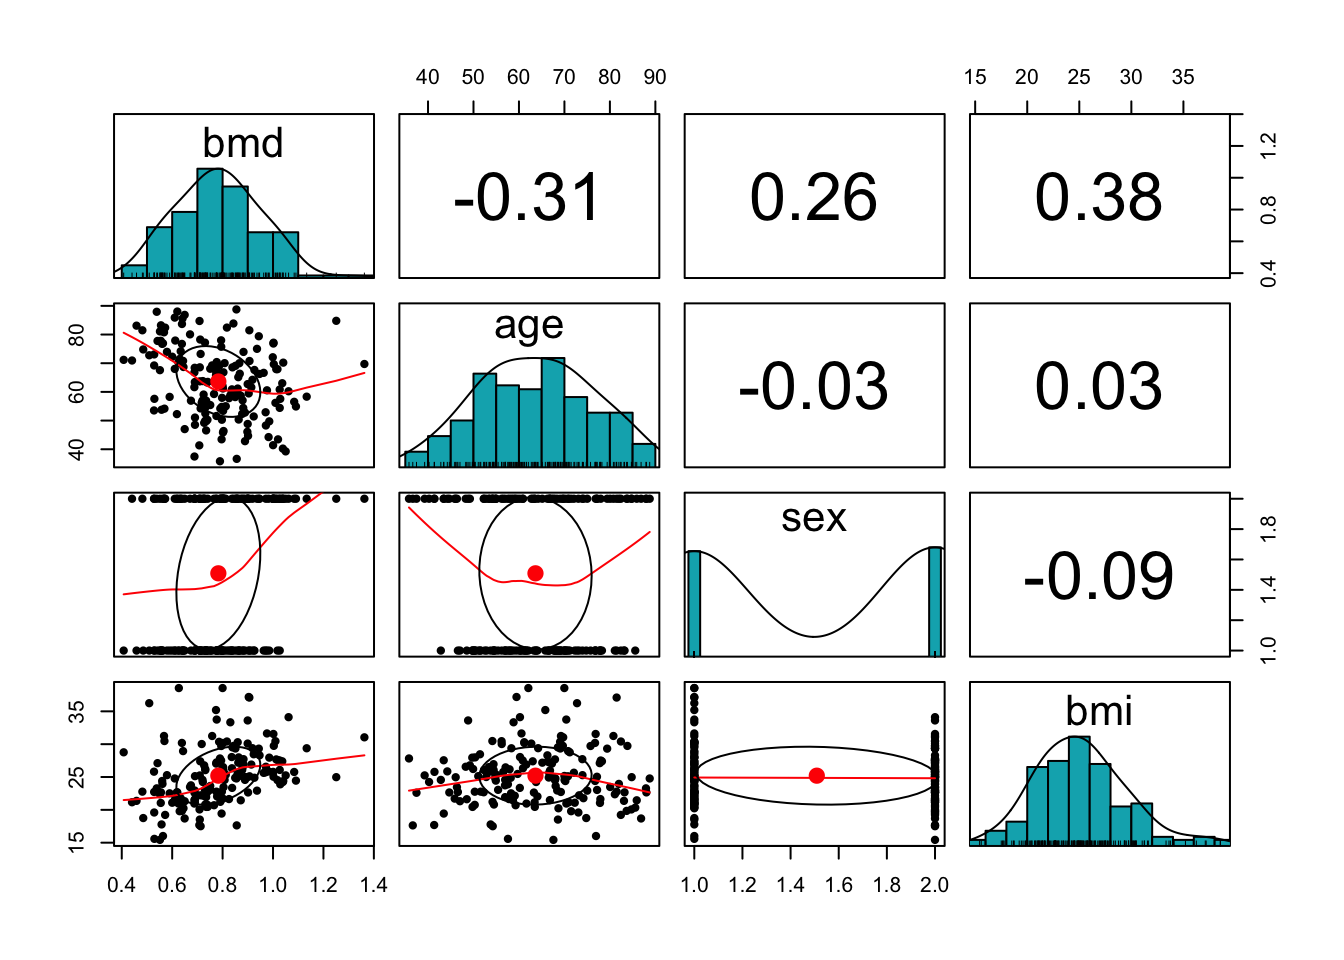
\includegraphics[keepaspectratio]{_main_files/figure-latex/unnamed-chunk-3-1.pdf}}

We fit a linear model for BMD and evaluate the R-squared

\begin{Shaded}
\begin{Highlighting}[]
\CommentTok{\#Fits a linear model with fixed effects only  }
\NormalTok{  model1.bmd }\OtherTok{\textless{}{-}} \FunctionTok{lm}\NormalTok{(bmd }\SpecialCharTok{\textasciitilde{}}\NormalTok{ age }\SpecialCharTok{+}\NormalTok{ sex }\SpecialCharTok{+}\NormalTok{ bmi, }\AttributeTok{data =}\NormalTok{ bmd.data)}
  \FunctionTok{summary}\NormalTok{(model1.bmd)}
\end{Highlighting}
\end{Shaded}

\begin{verbatim}
## 
## Call:
## lm(formula = bmd ~ age + sex + bmi, data = bmd.data)
## 
## Residuals:
##      Min       1Q   Median       3Q      Max 
## -0.38207 -0.07669 -0.00654  0.07888  0.51256 
## 
## Coefficients:
##               Estimate Std. Error t value Pr(>|t|)    
## (Intercept)  0.6063945  0.0834051   7.270 1.36e-11 ***
## age         -0.0041579  0.0008625  -4.821 3.23e-06 ***
## sexM         0.0949602  0.0213314   4.452 1.56e-05 ***
## bmi          0.0155913  0.0024239   6.432 1.30e-09 ***
## ---
## Signif. codes:  0 '***' 0.001 '**' 0.01 '*' 0.05 '.' 0.1 ' ' 1
## 
## Residual standard error: 0.138 on 165 degrees of freedom
## Multiple R-squared:  0.3254, Adjusted R-squared:  0.3131 
## F-statistic: 26.53 on 3 and 165 DF,  p-value: 4.677e-14
\end{verbatim}

\begin{Shaded}
\begin{Highlighting}[]
  \FunctionTok{mean}\NormalTok{(model1.bmd}\SpecialCharTok{$}\NormalTok{residuals}\SpecialCharTok{\^{}}\DecValTok{2}\NormalTok{) }\CommentTok{\#MSE}
\end{Highlighting}
\end{Shaded}

\begin{verbatim}
## [1] 0.01859697
\end{verbatim}

\textbf{TRY IT YOURSELF:}

\begin{enumerate}
\def\labelenumi{\arabic{enumi})}
\tightlist
\item
  Fit a linear model with the interaction age*sex - call it model 2
\end{enumerate}

\emph{See the solution code}

\begin{Shaded}
\begin{Highlighting}[]
\CommentTok{\#Fits a linear model with an interaction age*sex}
\NormalTok{  model2.bmd }\OtherTok{\textless{}{-}} \FunctionTok{lm}\NormalTok{(bmd }\SpecialCharTok{\textasciitilde{}}\NormalTok{ age }\SpecialCharTok{*}\NormalTok{ sex }\SpecialCharTok{+}\NormalTok{ bmi, }\AttributeTok{data =}\NormalTok{ bmd.data)}
  \FunctionTok{summary}\NormalTok{(model2.bmd)}
  \FunctionTok{mean}\NormalTok{(model2.bmd}\SpecialCharTok{$}\NormalTok{residuals}\SpecialCharTok{\^{}}\DecValTok{2}\NormalTok{) }\CommentTok{\#MSE}
\end{Highlighting}
\end{Shaded}

\begin{enumerate}
\def\labelenumi{\arabic{enumi}.}
\setcounter{enumi}{1}
\tightlist
\item
  Fit a linear model with the the interaction age*sex and cubic effect for
  BMI - call it model 3
\end{enumerate}

See the solution code

\begin{Shaded}
\begin{Highlighting}[]
\CommentTok{\#Fits a linear model with an interaction and polynomial f}
\NormalTok{  model3.bmd }\OtherTok{\textless{}{-}} \FunctionTok{lm}\NormalTok{(bmd }\SpecialCharTok{\textasciitilde{}}\NormalTok{ age}\SpecialCharTok{*}\NormalTok{sex  }\SpecialCharTok{+}\NormalTok{ bmi }\SpecialCharTok{+} \FunctionTok{I}\NormalTok{(bmi}\SpecialCharTok{\^{}}\DecValTok{2}\NormalTok{) }\SpecialCharTok{+} \FunctionTok{I}\NormalTok{(bmi}\SpecialCharTok{\^{}}\DecValTok{3}\NormalTok{), }
                   \AttributeTok{data =}\NormalTok{ bmd.data)}

  \CommentTok{\#You could use the poly() function to fit the same model}
  \CommentTok{\#however, poly() will use orthogonal polynomials}
  \CommentTok{\#so the coefficients will not be the same as above}
  \CommentTok{\#summary(lm(bmd \textasciitilde{} age*sex  + poly(bmi,3) , data = bmd.data))}
  \FunctionTok{summary}\NormalTok{(model3.bmd)}
  \FunctionTok{mean}\NormalTok{(model3.bmd}\SpecialCharTok{$}\NormalTok{residuals}\SpecialCharTok{\^{}}\DecValTok{2}\NormalTok{) }\CommentTok{\#MSE}
\end{Highlighting}
\end{Shaded}

\subsection*{Task 2 - Predicting from a linear model}\label{task-2---predicting-from-a-linear-model}
\addcontentsline{toc}{subsection}{Task 2 - Predicting from a linear model}

We first plot the scatter for BMD and BMI, then get the predictions from
model 3 in task 1, for a new data where age=50, sex=F and we let BMI
vary from 15 to 40. We also compute the predictions for males with similar
characteristics. Finally, we add the fitted lines to the plot.

\begin{Shaded}
\begin{Highlighting}[]
\CommentTok{\#Scatter plot of BMD and BMI}
  \FunctionTok{plot}\NormalTok{(bmd.data}\SpecialCharTok{$}\NormalTok{bmi, bmd.data}\SpecialCharTok{$}\NormalTok{bmd, }
        \AttributeTok{col =} \FunctionTok{ifelse}\NormalTok{(bmd.data}\SpecialCharTok{$}\NormalTok{sex}\SpecialCharTok{==}\StringTok{"F"}\NormalTok{, }\StringTok{"red"}\NormalTok{, }\StringTok{"blue"}\NormalTok{))}
\CommentTok{\#prediction from model b) in task 1}
\NormalTok{  bmd.f50 }\OtherTok{\textless{}{-}} \FunctionTok{predict}\NormalTok{(model3.bmd, }
                   \AttributeTok{newdata =} \FunctionTok{data.frame}\NormalTok{(}\AttributeTok{age=}\DecValTok{50}\NormalTok{, }\AttributeTok{sex=}\StringTok{"F"}\NormalTok{, }\AttributeTok{bmi=}\FunctionTok{seq}\NormalTok{(}\DecValTok{15}\NormalTok{,}\DecValTok{40}\NormalTok{)))}
\NormalTok{  bmd.m50 }\OtherTok{\textless{}{-}} \FunctionTok{predict}\NormalTok{(model3.bmd, }
                   \AttributeTok{newdata =} \FunctionTok{data.frame}\NormalTok{(}\AttributeTok{age=}\DecValTok{50}\NormalTok{, }\AttributeTok{sex=}\StringTok{"M"}\NormalTok{, }\AttributeTok{bmi=}\FunctionTok{seq}\NormalTok{(}\DecValTok{15}\NormalTok{,}\DecValTok{40}\NormalTok{)))}
  \FunctionTok{lines}\NormalTok{(}\FunctionTok{seq}\NormalTok{(}\DecValTok{15}\NormalTok{,}\DecValTok{40}\NormalTok{), bmd.f50, }\AttributeTok{col=}\StringTok{"red"}\NormalTok{)}
  \FunctionTok{lines}\NormalTok{(}\FunctionTok{seq}\NormalTok{(}\DecValTok{15}\NormalTok{,}\DecValTok{40}\NormalTok{), bmd.m50, }\AttributeTok{col=}\StringTok{"blue"}\NormalTok{)}
\end{Highlighting}
\end{Shaded}

\pandocbounded{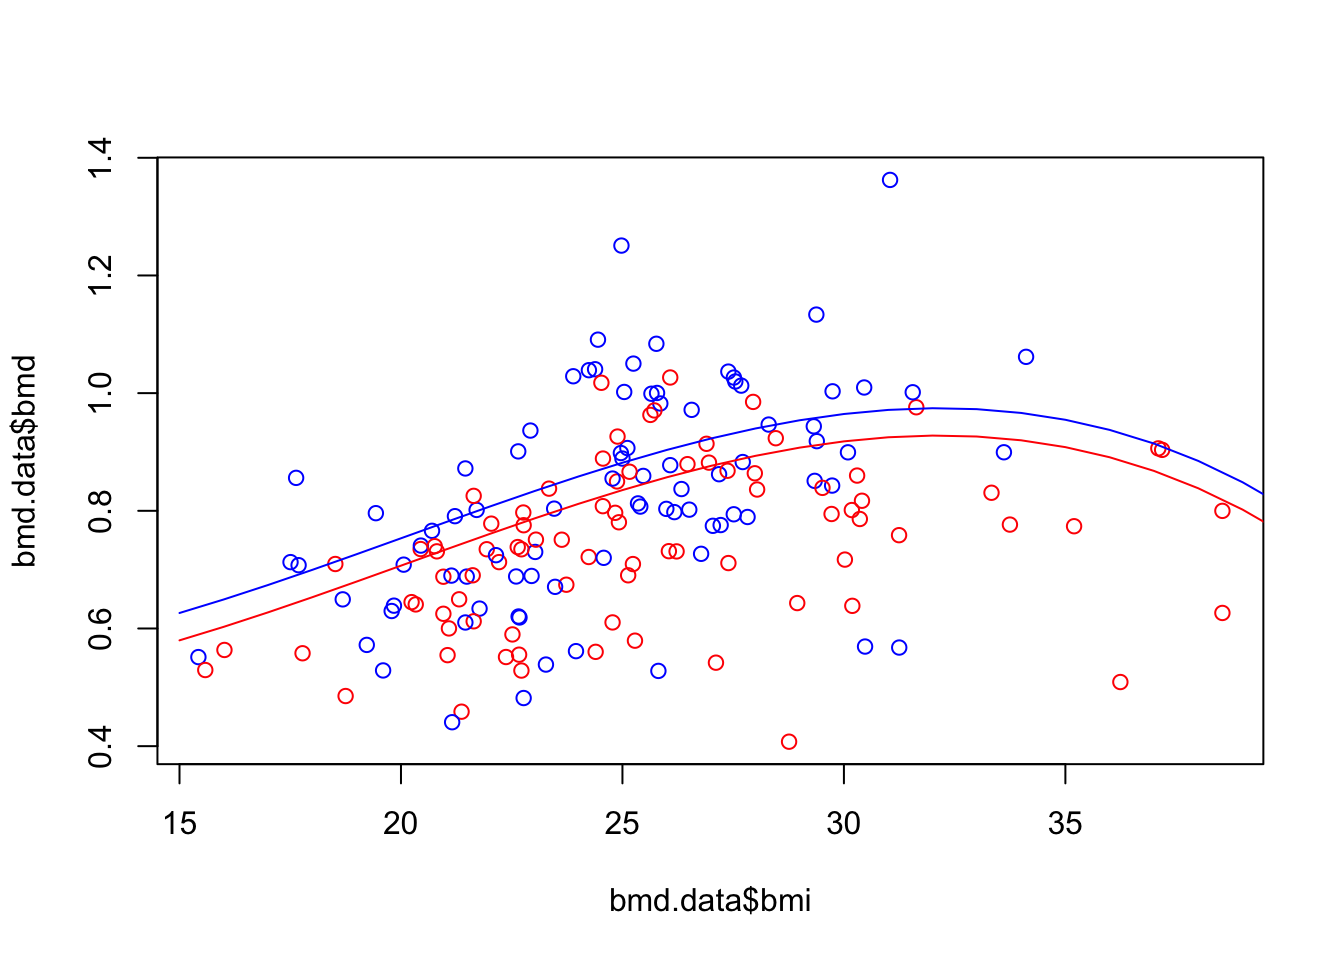
\includegraphics[keepaspectratio]{_main_files/figure-latex/BMDBMI-1.pdf}}

\textbf{TRY IT YOURSELF:}

\begin{enumerate}
\def\labelenumi{\arabic{enumi})}
\tightlist
\item
  Produce the scatter plot for BMD and AGE, only for women
\end{enumerate}

See the solution code

\begin{Shaded}
\begin{Highlighting}[]
\CommentTok{\#Scatter plot of BMD and AGE}
  \FunctionTok{plot}\NormalTok{( bmd.data}\SpecialCharTok{$}\NormalTok{age[bmd.data}\SpecialCharTok{$}\NormalTok{sex}\SpecialCharTok{==}\StringTok{"F"}\NormalTok{], bmd.data}\SpecialCharTok{$}\NormalTok{bmd[bmd.data}\SpecialCharTok{$}\NormalTok{sex}\SpecialCharTok{==}\StringTok{"F"}\NormalTok{])}
\end{Highlighting}
\end{Shaded}

\pandocbounded{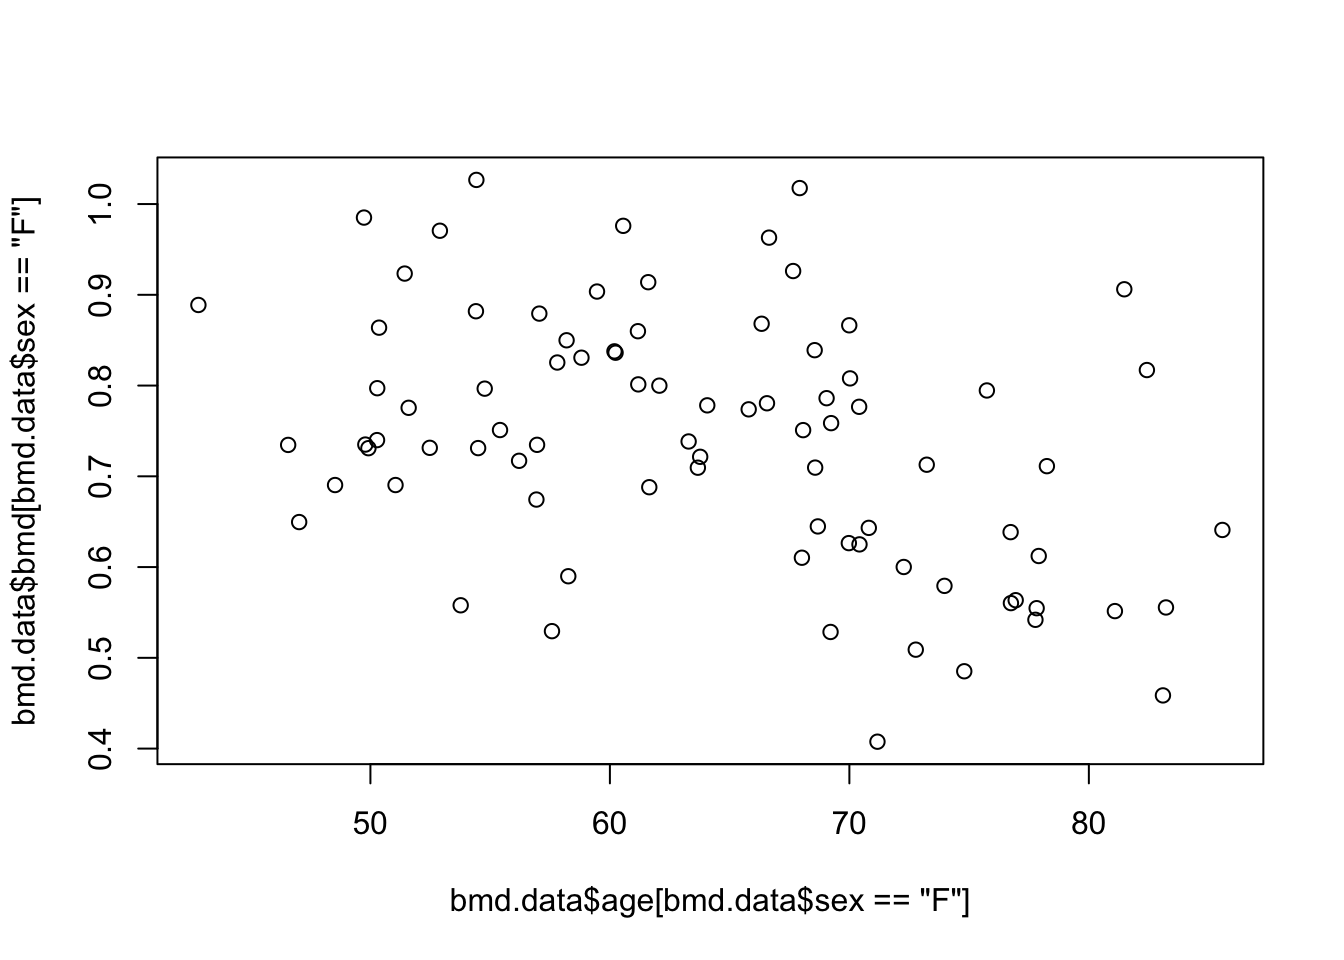
\includegraphics[keepaspectratio]{_main_files/figure-latex/BMDAGEWOMEN-1.pdf}}

\begin{enumerate}
\def\labelenumi{\arabic{enumi})}
\setcounter{enumi}{1}
\tightlist
\item
  Predict the BMD for women, with a BMI=25 and AGE between 40 and 90,
  using model 3 from task 1 and plot the prediction
\end{enumerate}

See the solution code

\begin{Shaded}
\begin{Highlighting}[]
\CommentTok{\#Scatter plot of BMD and AGE}
  \FunctionTok{plot}\NormalTok{( bmd.data}\SpecialCharTok{$}\NormalTok{age[bmd.data}\SpecialCharTok{$}\NormalTok{sex}\SpecialCharTok{==}\StringTok{"F"}\NormalTok{], bmd.data}\SpecialCharTok{$}\NormalTok{bmd[bmd.data}\SpecialCharTok{$}\NormalTok{sex}\SpecialCharTok{==}\StringTok{"F"}\NormalTok{])}

\CommentTok{\#prediction from model 3 in task 1}
\CommentTok{\#(the prediction line only )}
\NormalTok{  bmd.bmi25 }\OtherTok{\textless{}{-}} \FunctionTok{predict}\NormalTok{(model3.bmd, }
                   \AttributeTok{newdata =} \FunctionTok{data.frame}\NormalTok{(}\AttributeTok{age=}\FunctionTok{seq}\NormalTok{(}\DecValTok{40}\NormalTok{,}\DecValTok{90}\NormalTok{), }\AttributeTok{sex=}\StringTok{"F"}\NormalTok{, }\AttributeTok{bmi=}\DecValTok{25}\NormalTok{))}
  \FunctionTok{lines}\NormalTok{(}\FunctionTok{seq}\NormalTok{(}\DecValTok{40}\NormalTok{,}\DecValTok{90}\NormalTok{), bmd.bmi25)}
\end{Highlighting}
\end{Shaded}

\pandocbounded{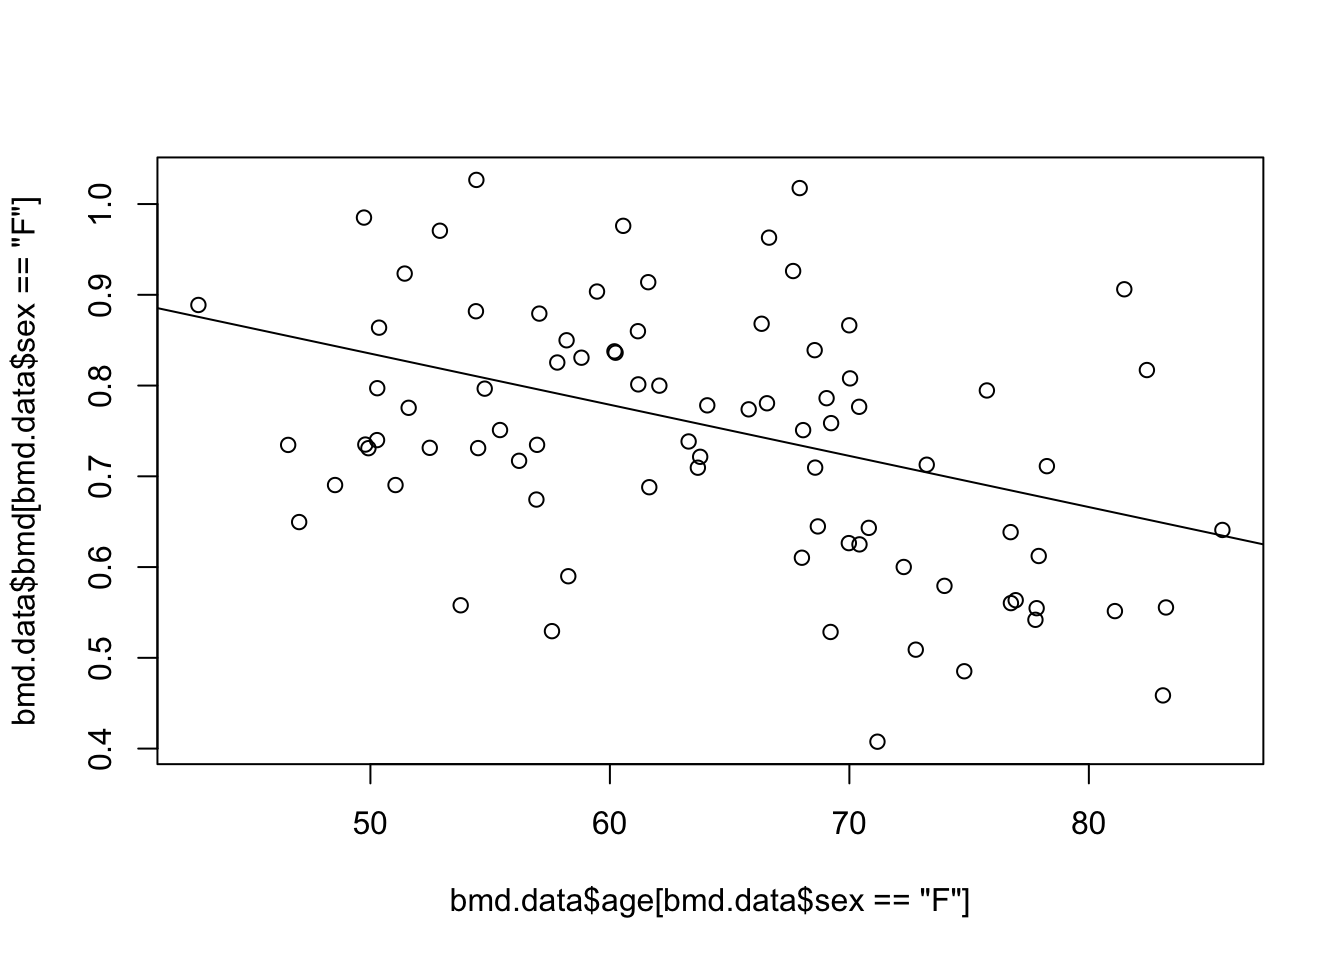
\includegraphics[keepaspectratio]{_main_files/figure-latex/BMDBMIpred -1.pdf}}

\section{Exercises}\label{LR.exerc}

Solve the following exercises from the \emph{An introduction to statistical learning} book:

\begin{enumerate}
\def\labelenumi{\arabic{enumi})}
\item
  Exercise 4 (page 122)
\item
  Exercise 13 (page 126)
\item
  With the \emph{fat} dataset in the \texttt{library(faraway)}, we want to
  fit a linear model to predict body fat (variable \textbf{brozek}) using the variable
  \textbf{abdom} and \textbf{age}. After loading the library, use the command \texttt{data(fat)}
  to load the dataset.

  \begin{enumerate}
  \def\labelenumii{\alph{enumii})}
  \item
    recode the variable age into \textbf{age\_cat} with the following categories:
    \textless30, 30-50 and \textgreater50
  \item
    fit a linear model using \textbf{abdom} and \textbf{age\_cat} and compute the mean
    squared error
  \item
    fit a linear model using \textbf{abdom} , \textbf{age\_cat} and the interaction
    between these two predictors. Comment on the change in the mean
    squared error of this model compared to the one without the interaction.
  \end{enumerate}
\end{enumerate}

\chapter{K-nearest Neighbours Regression}\label{k-nearest-neighbours-regression}

\section{Introduction}\label{knn.intro}

KNN regression is a non-parametric method that, in an intuitive manner,
approximates the association between independent variables and the continuous
outcome by
averaging the observations in the same \emph{neighbourhood}. The size of the
neighbourhood needs
to be set by the analyst or can be chosen using cross-validation (we will
see this later) to select the size that minimises the
mean-squared error.

While the method is quite appealing, it quickly becomes impractical when the
dimension increases, i.e., when there are many independent variables.

\section{Readings}\label{knn.read}

Read the following chapter of \emph{An introduction to statistical learning}:

\begin{itemize}
\tightlist
\item
  \href{https://static1.squarespace.com/static/5ff2adbe3fe4fe33db902812/t/6062a083acbfe82c7195b27d/1617076404560/ISLR\%2BSeventh\%2BPrinting.pdf}{3.5 Comparison of Linear Regression with K-Nearest Neighbors}
\end{itemize}

\section{Practical session}\label{knn.prac}

\subsection*{Task - Fit a knn regression}\label{task---fit-a-knn-regression}
\addcontentsline{toc}{subsection}{Task - Fit a knn regression}

With the \href{https://www.dropbox.com/s/7wjsfdaf0wt2kg2/bmd.csv?dl=1}{bmd.csv} dataset, we want to fit a knn regression with k=3 for BMD,
with age as covariates. Then we will compute the MSE and \(R^2\).

\begin{Shaded}
\begin{Highlighting}[]
\CommentTok{\#libraries that we will need}
\FunctionTok{library}\NormalTok{(FNN)   }\CommentTok{\#knn regression}
\end{Highlighting}
\end{Shaded}

\begin{verbatim}
## Warning: package 'FNN' was built under R version 4.3.3
\end{verbatim}

\begin{Shaded}
\begin{Highlighting}[]
\FunctionTok{set.seed}\NormalTok{(}\DecValTok{1974}\NormalTok{) }\CommentTok{\#fix the random generator seed }

\CommentTok{\#read the data}
\NormalTok{bmd.data     }\OtherTok{\textless{}{-}} 
  \FunctionTok{read.csv}\NormalTok{(}\StringTok{"https://www.dropbox.com/s/c6mhgatkotuze8o/bmd.csv?dl=1"}\NormalTok{, }
           \AttributeTok{stringsAsFactors =} \ConstantTok{TRUE}\NormalTok{)}
\end{Highlighting}
\end{Shaded}

\begin{Shaded}
\begin{Highlighting}[]
\CommentTok{\#Fit a knn regression with k=3}
\CommentTok{\#using the knn.reg() function from the FNN package}
\NormalTok{knn3.bmd }\OtherTok{\textless{}{-}} \FunctionTok{knn.reg}\NormalTok{(}\AttributeTok{train=}\NormalTok{bmd.data[}\FunctionTok{c}\NormalTok{(}\StringTok{"age"}\NormalTok{)],   }
                     \AttributeTok{y=}\NormalTok{bmd.data}\SpecialCharTok{$}\NormalTok{bmd, }
                     \AttributeTok{test=} \FunctionTok{data.frame}\NormalTok{(}\AttributeTok{age=}\FunctionTok{seq}\NormalTok{(}\DecValTok{38}\NormalTok{,}\DecValTok{89}\NormalTok{)),}
                     \AttributeTok{k=}\DecValTok{3}\NormalTok{)    }
\end{Highlighting}
\end{Shaded}

Before computing the MSE and \(R^2\), we will plot the model predictions

\begin{Shaded}
\begin{Highlighting}[]
  \FunctionTok{plot}\NormalTok{(bmd.data}\SpecialCharTok{$}\NormalTok{age, bmd.data}\SpecialCharTok{$}\NormalTok{bmd) }\CommentTok{\#adding the scatter for BMI and BMD}
  \FunctionTok{lines}\NormalTok{(}\FunctionTok{seq}\NormalTok{(}\DecValTok{38}\NormalTok{,}\DecValTok{89}\NormalTok{), knn3.bmd}\SpecialCharTok{$}\NormalTok{pred)  }\CommentTok{\#adds the knn k=3 line}
\end{Highlighting}
\end{Shaded}

\pandocbounded{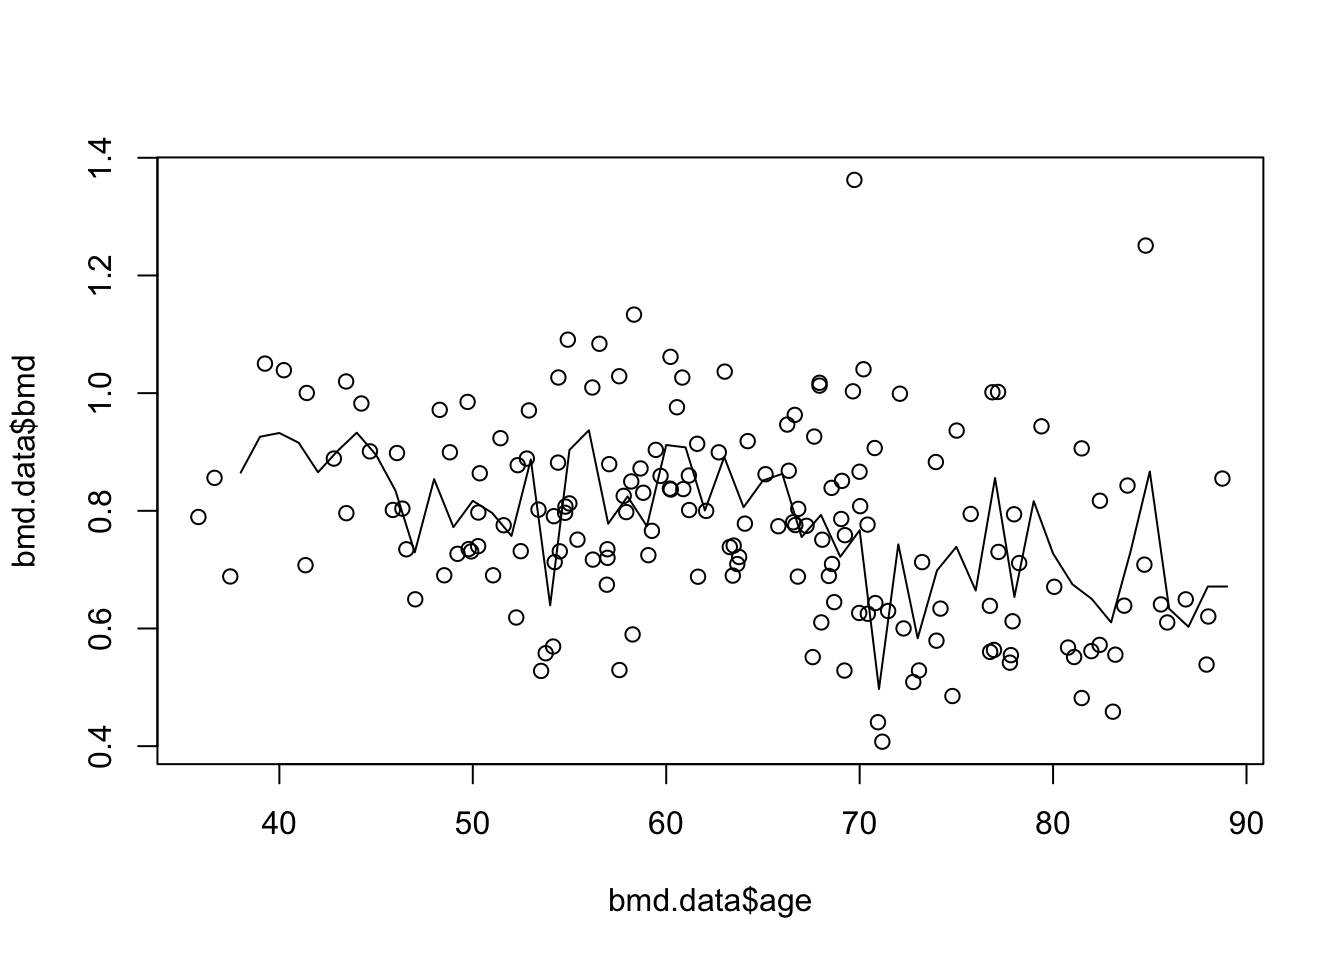
\includegraphics[keepaspectratio]{_main_files/figure-latex/agebmd-1.pdf}}

Finally, we compute the MSE and \(R^2\) for knn k=3. We have to refit the models and ``test'' them in the original data

\begin{Shaded}
\begin{Highlighting}[]
\NormalTok{  knn3.bmd.datapred }\OtherTok{\textless{}{-}} \FunctionTok{knn.reg}\NormalTok{(}\AttributeTok{train=}\NormalTok{bmd.data[}\FunctionTok{c}\NormalTok{(}\StringTok{"age"}\NormalTok{)],  }
                           \AttributeTok{y=}\NormalTok{bmd.data}\SpecialCharTok{$}\NormalTok{bmd, }
                           \AttributeTok{test=}\NormalTok{bmd.data[}\FunctionTok{c}\NormalTok{(}\StringTok{"age"}\NormalTok{)], }\CommentTok{\#ORIGINAL DATA}
                           \AttributeTok{k=}\DecValTok{3}\NormalTok{)      }\CommentTok{\#knn reg with k=3}
  \CommentTok{\#MSE for knn k=3 }
\NormalTok{  mse.knn3  }\OtherTok{\textless{}{-}} \FunctionTok{mean}\NormalTok{((knn3.bmd.datapred}\SpecialCharTok{$}\NormalTok{pred }\SpecialCharTok{{-}}\NormalTok{ bmd.data}\SpecialCharTok{$}\NormalTok{bmd)}\SpecialCharTok{\^{}}\DecValTok{2}\NormalTok{)  }
\NormalTok{  mse.knn3}
\end{Highlighting}
\end{Shaded}

\begin{verbatim}
## [1] 0.01531282
\end{verbatim}

\begin{Shaded}
\begin{Highlighting}[]
\NormalTok{  r2.knn3   }\OtherTok{\textless{}{-}} \DecValTok{1}\SpecialCharTok{{-}}\NormalTok{ mse.knn3}\SpecialCharTok{/}\NormalTok{(}\FunctionTok{var}\NormalTok{(bmd.data}\SpecialCharTok{$}\NormalTok{bmd)}\SpecialCharTok{*}\DecValTok{168}\SpecialCharTok{/}\DecValTok{169}\NormalTok{) }\CommentTok{\#R2 for knn k=3 using }
\NormalTok{  r2.knn3                                              }\CommentTok{\#R2 = 1{-}MSE/var(y)}
\end{Highlighting}
\end{Shaded}

\begin{verbatim}
## [1] 0.4445392
\end{verbatim}

\textbf{TRY IT YOURSELF:}

\begin{enumerate}
\def\labelenumi{\arabic{enumi})}
\tightlist
\item
  Fit a knn regression for BMD using AGE, with k=20
\end{enumerate}

\emph{See the solution code}

\begin{Shaded}
\begin{Highlighting}[]
\NormalTok{  knn20.bmd }\OtherTok{\textless{}{-}} \FunctionTok{knn.reg}\NormalTok{(}\AttributeTok{train=}\NormalTok{bmd.data[}\FunctionTok{c}\NormalTok{(}\StringTok{"age"}\NormalTok{)],   }
                      \AttributeTok{y=}\NormalTok{bmd.data}\SpecialCharTok{$}\NormalTok{bmd, }
                      \AttributeTok{test=} \FunctionTok{data.frame}\NormalTok{(}\AttributeTok{age=}\FunctionTok{seq}\NormalTok{(}\DecValTok{38}\NormalTok{,}\DecValTok{89}\NormalTok{)),}
                      \AttributeTok{k=}\DecValTok{20}\NormalTok{)     }\CommentTok{\#knn regression with k=20}
\end{Highlighting}
\end{Shaded}

\begin{enumerate}
\def\labelenumi{\arabic{enumi})}
\setcounter{enumi}{1}
\tightlist
\item
  Add the prediction line to the previous scatter plot
\end{enumerate}

\emph{See the solution code}

\begin{Shaded}
\begin{Highlighting}[]
\FunctionTok{plot}\NormalTok{(bmd.data}\SpecialCharTok{$}\NormalTok{age, bmd.data}\SpecialCharTok{$}\NormalTok{bmd) }\CommentTok{\#adding the scatter for BMI and BMD}
\FunctionTok{lines}\NormalTok{(}\FunctionTok{seq}\NormalTok{(}\DecValTok{38}\NormalTok{,}\DecValTok{89}\NormalTok{), knn3.bmd}\SpecialCharTok{$}\NormalTok{pred) }
\FunctionTok{lines}\NormalTok{(}\FunctionTok{seq}\NormalTok{(}\DecValTok{38}\NormalTok{,}\DecValTok{89}\NormalTok{), knn20.bmd}\SpecialCharTok{$}\NormalTok{pred, }\AttributeTok{col=}\StringTok{"blue"}\NormalTok{)  }\CommentTok{\#adds the knn k=20 gray line}
\end{Highlighting}
\end{Shaded}

\pandocbounded{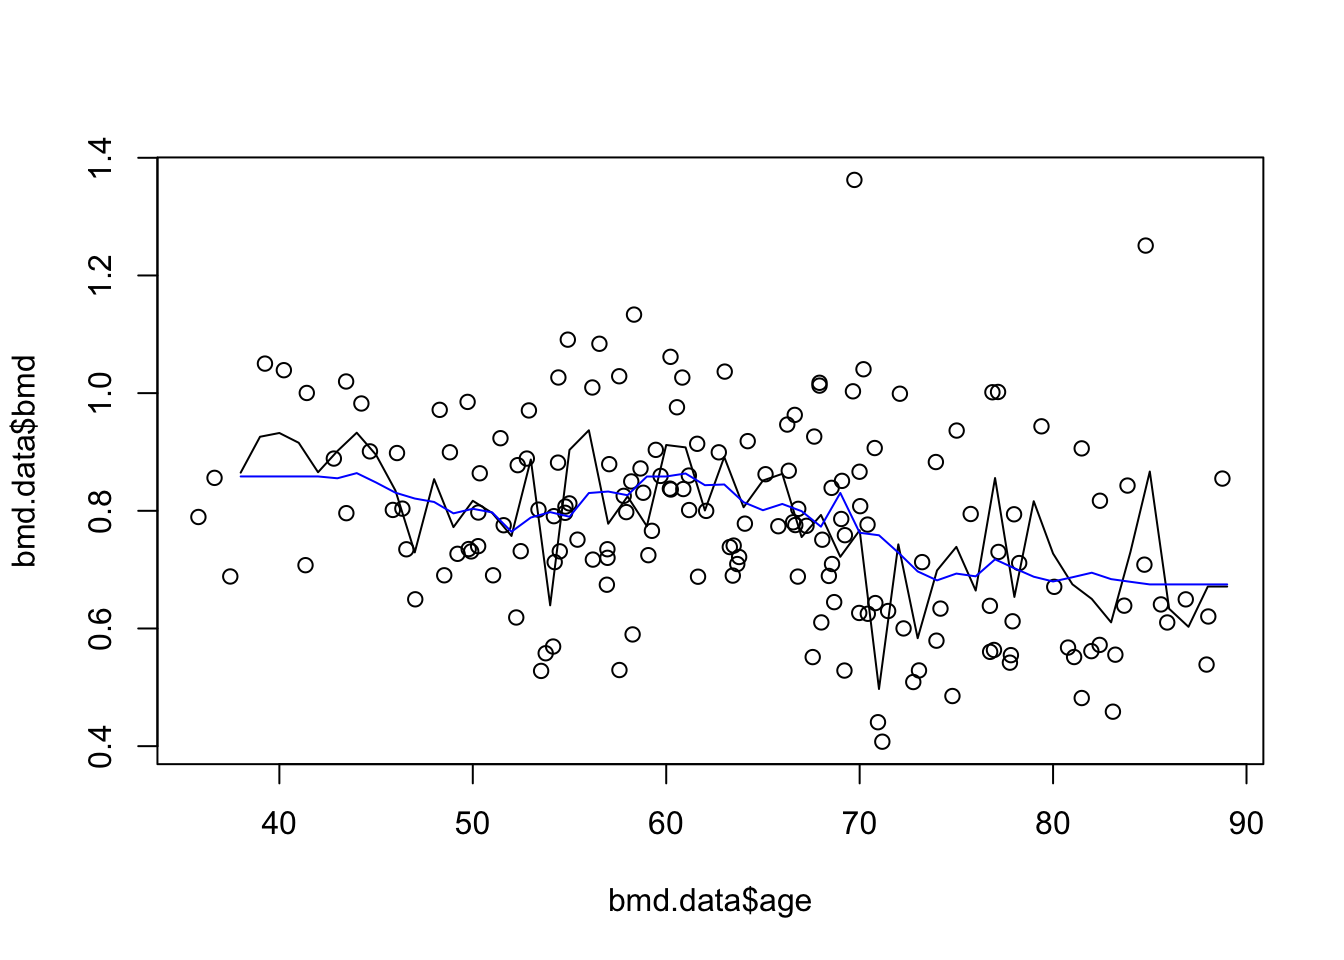
\includegraphics[keepaspectratio]{_main_files/figure-latex/knn3and20-1.pdf}}

\begin{enumerate}
\def\labelenumi{\arabic{enumi})}
\setcounter{enumi}{2}
\tightlist
\item
  Compute the MSE and \(R^2\)
\end{enumerate}

\emph{See the solution code}

\begin{Shaded}
\begin{Highlighting}[]
\CommentTok{\#predictions from knn reg with k=20}
\NormalTok{knn20.bmd.datapred }\OtherTok{\textless{}{-}} \FunctionTok{knn.reg}\NormalTok{(}
  \AttributeTok{train =}\NormalTok{ bmd.data[}\FunctionTok{c}\NormalTok{(}\StringTok{"age"}\NormalTok{)],}
  \AttributeTok{y =}\NormalTok{ bmd.data}\SpecialCharTok{$}\NormalTok{bmd,}
  \AttributeTok{test =}\NormalTok{ bmd.data[}\FunctionTok{c}\NormalTok{(}\StringTok{"age"}\NormalTok{)],}
  \CommentTok{\#ORIGINAL DATA}
  \AttributeTok{k =} \DecValTok{20}
\NormalTok{)    }

\CommentTok{\#MSE for knn k=20}
\NormalTok{mse.knn20 }\OtherTok{\textless{}{-}} \FunctionTok{mean}\NormalTok{((knn20.bmd.datapred}\SpecialCharTok{$}\NormalTok{pred }\SpecialCharTok{{-}}\NormalTok{ bmd.data}\SpecialCharTok{$}\NormalTok{bmd) }\SpecialCharTok{\^{}} \DecValTok{2}\NormalTok{) }
\NormalTok{mse.knn20}

\CommentTok{\#r2 for knn k=20}
\NormalTok{r2.knn20 }\OtherTok{\textless{}{-}} \DecValTok{1}\SpecialCharTok{{-}}\NormalTok{mse.knn20}\SpecialCharTok{/}\NormalTok{(}\FunctionTok{var}\NormalTok{(bmd.data}\SpecialCharTok{$}\NormalTok{bmd)}\SpecialCharTok{*}\DecValTok{168}\SpecialCharTok{/}\DecValTok{169}\NormalTok{) }\CommentTok{\#168/169 is added to correct }
\NormalTok{r2.knn20                                              }\CommentTok{\#the degrees of freedom}
\end{Highlighting}
\end{Shaded}

\begin{enumerate}
\def\labelenumi{\arabic{enumi})}
\setcounter{enumi}{3}
\tightlist
\item
  Add a linear prediction for BMD using AGE to the scatter plot
\end{enumerate}

\emph{See the solution code}

\begin{Shaded}
\begin{Highlighting}[]
\CommentTok{\#The initial plot with knn3 and knn20}
\FunctionTok{plot}\NormalTok{(bmd.data}\SpecialCharTok{$}\NormalTok{age, bmd.data}\SpecialCharTok{$}\NormalTok{bmd) }\CommentTok{\#adding the scatter for BMI and BMD}
\FunctionTok{lines}\NormalTok{(}\FunctionTok{seq}\NormalTok{(}\DecValTok{38}\NormalTok{,}\DecValTok{89}\NormalTok{), knn3.bmd}\SpecialCharTok{$}\NormalTok{pred) }
\FunctionTok{lines}\NormalTok{(}\FunctionTok{seq}\NormalTok{(}\DecValTok{38}\NormalTok{,}\DecValTok{89}\NormalTok{), knn20.bmd}\SpecialCharTok{$}\NormalTok{pred, }\AttributeTok{col=}\StringTok{"blue"}\NormalTok{)  }\CommentTok{\#adds the knn k=20 gray line}
  
\CommentTok{\#linear model and predictions  }
\NormalTok{model.age }\OtherTok{\textless{}{-}} \FunctionTok{lm}\NormalTok{(bmd }\SpecialCharTok{\textasciitilde{}}\NormalTok{ age, }
                   \AttributeTok{data =}\NormalTok{ bmd.data)}
\NormalTok{bmd.pred }\OtherTok{\textless{}{-}} \FunctionTok{predict}\NormalTok{(model.age, }
                   \AttributeTok{newdata =} \FunctionTok{data.frame}\NormalTok{(}\AttributeTok{age=}\FunctionTok{seq}\NormalTok{(}\DecValTok{38}\NormalTok{,}\DecValTok{89}\NormalTok{)))}
\FunctionTok{lines}\NormalTok{(}\FunctionTok{seq}\NormalTok{(}\DecValTok{38}\NormalTok{,}\DecValTok{89}\NormalTok{), bmd.pred) }\CommentTok{\#add the linear predictions to the plot}
\end{Highlighting}
\end{Shaded}

\pandocbounded{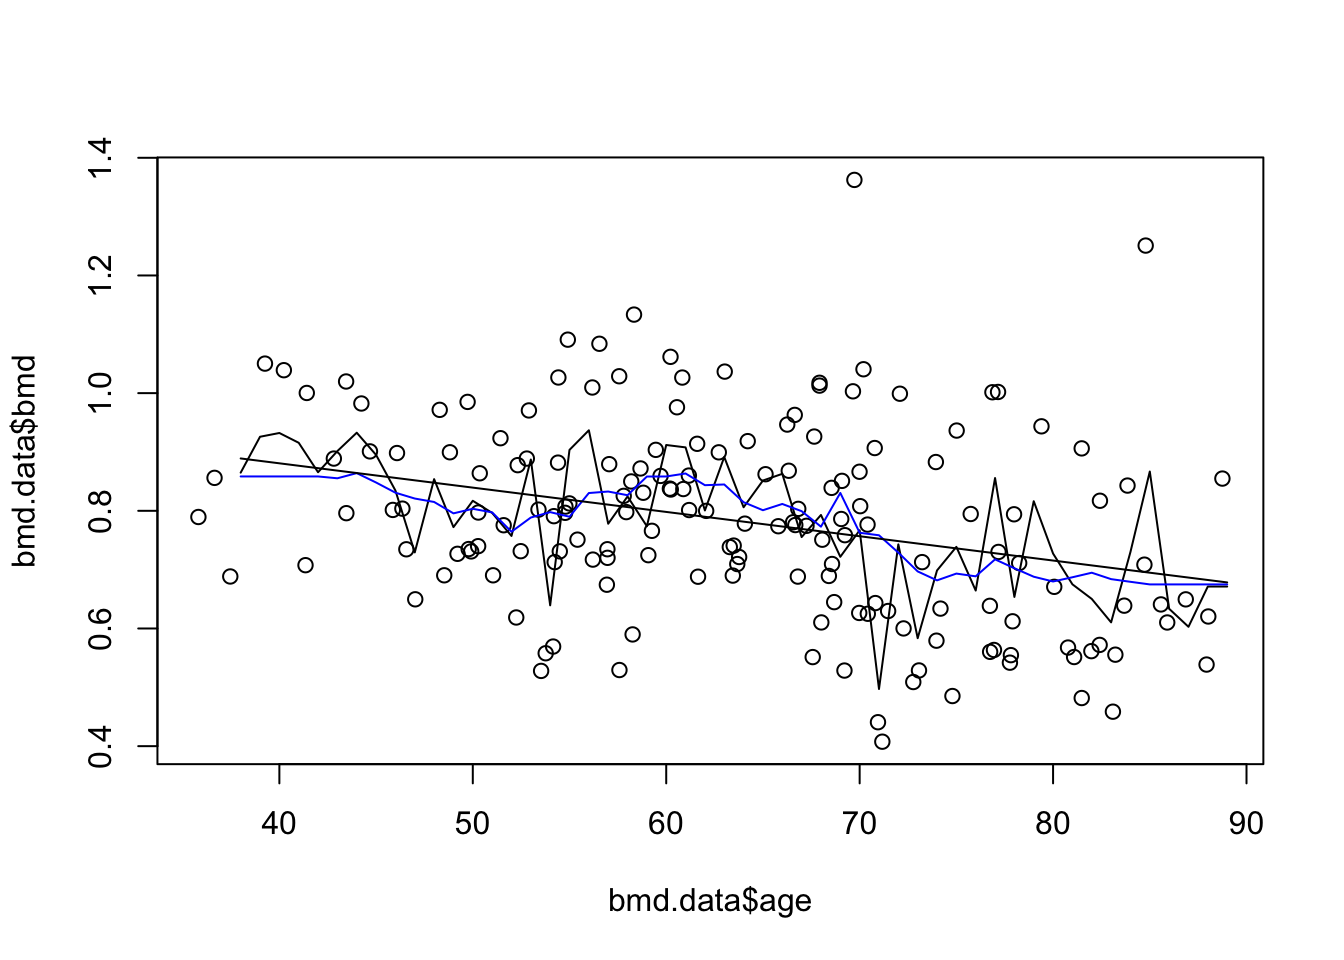
\includegraphics[keepaspectratio]{_main_files/figure-latex/knn3and20andlinear-1.pdf}}

\section{Exercises}\label{knn.exerc}

\begin{enumerate}
\def\labelenumi{\arabic{enumi})}
\item
  With the \emph{fat} dataset in the \emph{library(faraway)}, we want to predict body
  fat (variable \textbf{brozek}) using the variable \textbf{abdom}

  \begin{enumerate}
  \def\labelenumii{\alph{enumii})}
  \item
    use a k-nearest neighbour regression, with k=3,5 and 11, to approximate
    the relation between \textbf{brozek} and \textbf{abdom}. Plot the three lines.
  \item
    What is the predicted \textbf{brozek} for someone with \textbf{abdom=90} using
    knn=11?
  \item
    What is the predicted \textbf{brozek} for someone with \textbf{abdom=90} using a
    linear model?
  \item
    Compute the mean squared error for k=3,5 and 11
  \end{enumerate}
\item
  With the same data \emph{fat}, use a knn (k=9) to predict body
  fat (variable \textbf{brozek}) using the variables \textbf{abdom} and \textbf{age}
\end{enumerate}

\begin{enumerate}
\def\labelenumi{\alph{enumi})}
\item
  Plot the predictions for \textbf{abdom = 80 to 115} and \textbf{age = 30}
\item
  Would you expect the mean squared error for k=1 to be greater or smaller
  than the one for k=9? Why would you prefer k=9 over k=1?
\end{enumerate}

\chapter{Logistic regression}\label{logistic-regression}

\section{Introduction}\label{lr.intro}

You should also be familiar with logistic regression but not necessarily
as a classification method. In this section, we will see how this model can
be used to make predictions for categorical outcomes.
Like the linear model, there will be several
aspects, such as hypothesis testing, that we will not discussed in detail.

\section{Readings}\label{lr.read}

Read the following chapters of \emph{An introduction to statistical learning}:

\begin{itemize}
\tightlist
\item
  4.2 Why not Linear Regression?
\item
  4.3 Logistic Regression
\item
  Read about the \emph{Confusion Matrix} and \emph{ROC curve} in the
  subchapter 4.4.2
\end{itemize}

\section{Practical session}\label{lr.prac}

\subsection*{Task - Logistic regression}\label{task---logistic-regression}
\addcontentsline{toc}{subsection}{Task - Logistic regression}

With the \href{https://www.dropbox.com/s/7wjsfdaf0wt2kg2/bmd.csv?dl=1}{bmd.csv}
dataset, let's fit a logistic regression model to predict fracture, using AGE,
SEX, BMI and BMD as main effects.

\begin{Shaded}
\begin{Highlighting}[]
\CommentTok{\#libraries that we will need}
\FunctionTok{library}\NormalTok{(pROC) }\CommentTok{\#ROC curve}
\FunctionTok{set.seed}\NormalTok{(}\DecValTok{1974}\NormalTok{) }\CommentTok{\#fix the random generator seed }

\CommentTok{\#read the data}
\NormalTok{bmd.data     }\OtherTok{\textless{}{-}} 
  \FunctionTok{read.csv}\NormalTok{(}\StringTok{"https://www.dropbox.com/s/c6mhgatkotuze8o/bmd.csv?dl=1"}\NormalTok{, }
           \AttributeTok{stringsAsFactors =} \ConstantTok{TRUE}\NormalTok{)}
  
\NormalTok{bmd.data}\SpecialCharTok{$}\NormalTok{bmi }\OtherTok{\textless{}{-}}\NormalTok{ bmd.data}\SpecialCharTok{$}\NormalTok{weight\_kg }\SpecialCharTok{/}\NormalTok{ (bmd.data}\SpecialCharTok{$}\NormalTok{height\_cm}\SpecialCharTok{/}\DecValTok{100}\NormalTok{)}\SpecialCharTok{\^{}}\DecValTok{2}
\end{Highlighting}
\end{Shaded}

\begin{Shaded}
\begin{Highlighting}[]
\CommentTok{\#Fits a logistic model with fixed effects only  }
\NormalTok{  model1.fracture }\OtherTok{\textless{}{-}} \FunctionTok{glm}\NormalTok{(fracture}\SpecialCharTok{==}\StringTok{"fracture"} \SpecialCharTok{\textasciitilde{}}\NormalTok{ age }\SpecialCharTok{+}\NormalTok{ sex }\SpecialCharTok{+}\NormalTok{ bmi }\SpecialCharTok{+}\NormalTok{ bmd, }
                         \AttributeTok{family=}\NormalTok{binomial, }\AttributeTok{data =}\NormalTok{ bmd.data)}
  \FunctionTok{summary}\NormalTok{(model1.fracture)}
\end{Highlighting}
\end{Shaded}

\begin{verbatim}
## 
## Call:
## glm(formula = fracture == "fracture" ~ age + sex + bmi + bmd, 
##     family = binomial, data = bmd.data)
## 
## Coefficients:
##              Estimate Std. Error z value Pr(>|z|)    
## (Intercept)   9.79488    2.69720   3.631 0.000282 ***
## age           0.01844    0.02094   0.881 0.378540    
## sexM          0.84599    0.51249   1.651 0.098792 .  
## bmi          -0.05131    0.06013  -0.853 0.393537    
## bmd         -15.11747    2.80337  -5.393 6.94e-08 ***
## ---
## Signif. codes:  0 '***' 0.001 '**' 0.01 '*' 0.05 '.' 0.1 ' ' 1
## 
## (Dispersion parameter for binomial family taken to be 1)
## 
##     Null deviance: 205.27  on 168  degrees of freedom
## Residual deviance: 110.86  on 164  degrees of freedom
## AIC: 120.86
## 
## Number of Fisher Scoring iterations: 6
\end{verbatim}

We will use a Bayes classifier threshold (pred prob \textless.5) to classify each
patient and then check the misclassifications using the confusion matrix.

\begin{Shaded}
\begin{Highlighting}[]
\CommentTok{\#for model1}
\NormalTok{model1.fracture.pred }\OtherTok{\textless{}{-}} \FunctionTok{predict}\NormalTok{(model1.fracture,      }\CommentTok{\#probabilities }
                                \AttributeTok{type=}\StringTok{"response"}\NormalTok{)      }\CommentTok{\#predicted by the model}

\CommentTok{\#if prob\textgreater{}.5 returns TRUE (fracture)                  }
\NormalTok{model1.fracture.class }\OtherTok{\textless{}{-}}\NormalTok{ model1.fracture.pred }\SpecialCharTok{\textgreater{}}\NormalTok{ .}\DecValTok{5}    

\CommentTok{\#now build the confusion matrix}
\FunctionTok{table}\NormalTok{(model1.fracture.class, bmd.data}\SpecialCharTok{$}\NormalTok{fracture)     }
\end{Highlighting}
\end{Shaded}

\begin{verbatim}
##                      
## model1.fracture.class fracture no fracture
##                 FALSE       15         110
##                 TRUE        35           9
\end{verbatim}

So, from the table above you can see that based on the cut-off for
the predictive probability of 0.5, the model predicted 35 out of
the 50 fractures. And it predicted 110 out of the 119 no fractures.

Let's now plot the ROC and calculate the area under the curve. There are
several packages in R to do this; we will be using the library pROC.

\begin{Shaded}
\begin{Highlighting}[]
\NormalTok{  auc.model1.fracture }\OtherTok{\textless{}{-}} \FunctionTok{roc}\NormalTok{(fracture }\SpecialCharTok{\textasciitilde{}}\NormalTok{ model1.fracture.pred, }\CommentTok{\#using the pred prob}
                             \AttributeTok{data =}\NormalTok{ bmd.data)                 }\CommentTok{\#from the model}
\end{Highlighting}
\end{Shaded}

\begin{verbatim}
## Setting levels: control = fracture, case = no fracture
\end{verbatim}

\begin{verbatim}
## Setting direction: controls > cases
\end{verbatim}

\begin{Shaded}
\begin{Highlighting}[]
\NormalTok{  auc.model1.fracture}
\end{Highlighting}
\end{Shaded}

\begin{verbatim}
## 
## Call:
## roc.formula(formula = fracture ~ model1.fracture.pred, data = bmd.data)
## 
## Data: model1.fracture.pred in 50 controls (fracture fracture) > 119 cases (fracture no fracture).
## Area under the curve: 0.9195
\end{verbatim}

\begin{Shaded}
\begin{Highlighting}[]
  \FunctionTok{plot}\NormalTok{(auc.model1.fracture) }
  \FunctionTok{text}\NormalTok{(}\FloatTok{0.6}\NormalTok{,.}\DecValTok{6}\NormalTok{, }\FunctionTok{paste}\NormalTok{(}\StringTok{"AUC = "}\NormalTok{, }\FunctionTok{round}\NormalTok{(auc.model1.fracture}\SpecialCharTok{$}\NormalTok{auc,}\DecValTok{2}\NormalTok{)))}
\end{Highlighting}
\end{Shaded}

\pandocbounded{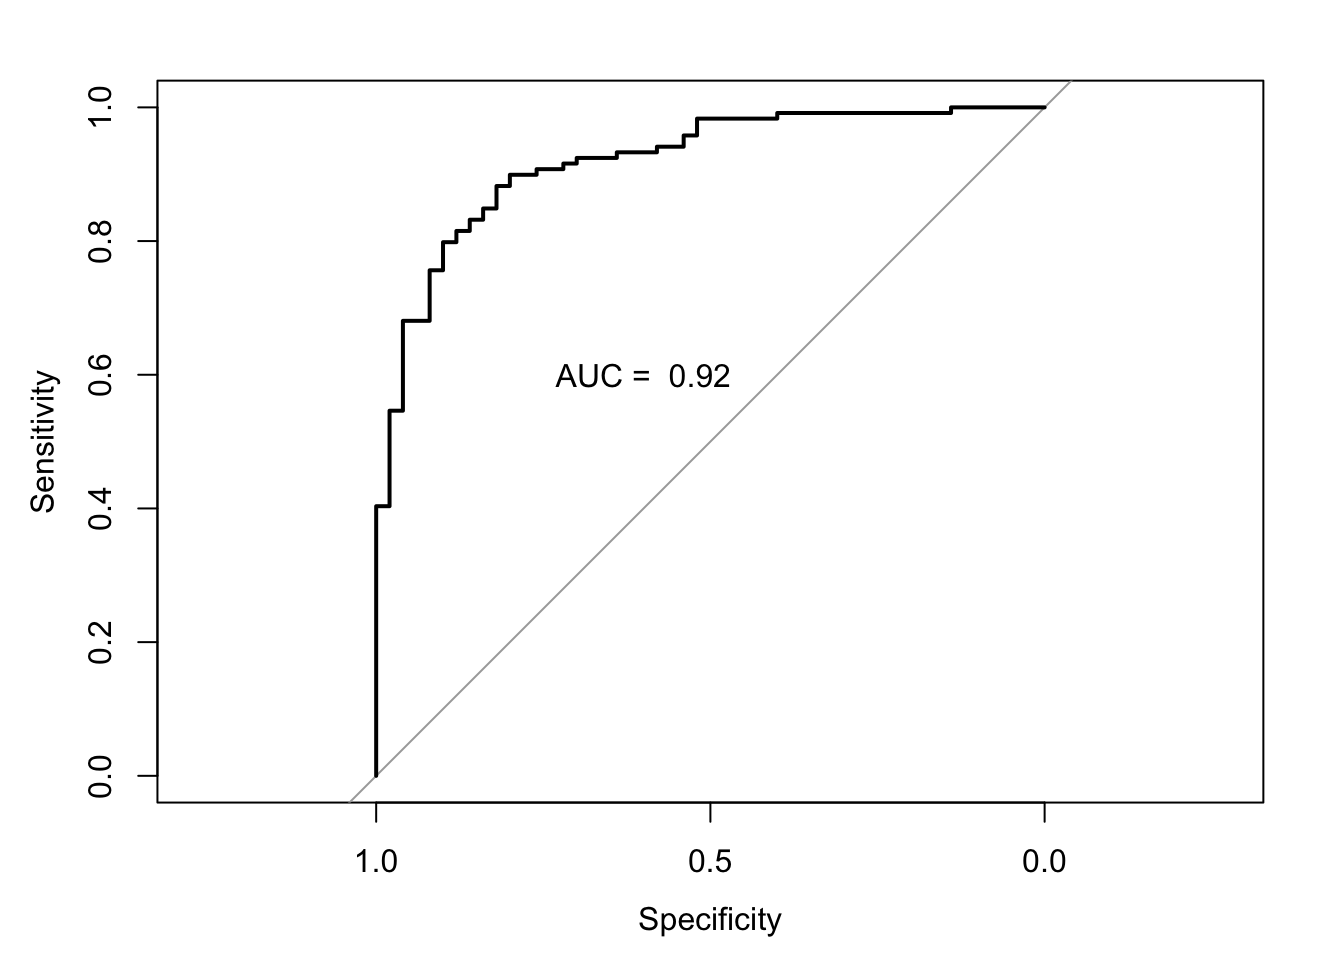
\includegraphics[keepaspectratio]{_main_files/figure-latex/unnamed-chunk-15-1.pdf}}

\textbf{TRY IT YOURSELF:}
1) Fit a similar model to model1.fracture but add a quadratic effect for age,
i.e., I(age\^{}2) and compare the AIC of both models.

\emph{See the solution code}

\begin{Shaded}
\begin{Highlighting}[]
\CommentTok{\#Fits a logistic model as model1.fracture but adds the quadratic effect for age}
\NormalTok{    model2.fracture }\OtherTok{\textless{}{-}} \FunctionTok{glm}\NormalTok{(fracture}\SpecialCharTok{==}\StringTok{"fracture"} \SpecialCharTok{\textasciitilde{}}\NormalTok{ age }\SpecialCharTok{+}  \FunctionTok{I}\NormalTok{(age}\SpecialCharTok{\^{}}\DecValTok{2}\NormalTok{) }\SpecialCharTok{+}\NormalTok{ bmi }\SpecialCharTok{+}
\NormalTok{                                                  sex }\SpecialCharTok{+}\NormalTok{ bmd,  }
                         \AttributeTok{family=}\NormalTok{binomial, }\AttributeTok{data =}\NormalTok{ bmd.data)}
    \FunctionTok{summary}\NormalTok{(model2.fracture)}
\end{Highlighting}
\end{Shaded}

\begin{enumerate}
\def\labelenumi{\arabic{enumi})}
\setcounter{enumi}{1}
\tightlist
\item
  Compute the classification error for the Bayes classifier using the confusion
  matrix.
\end{enumerate}

\emph{See the solution code}

\begin{Shaded}
\begin{Highlighting}[]
\CommentTok{\#Produce the confusion matrices for the models fitted}
\NormalTok{model2.fracture.pred }\OtherTok{\textless{}{-}} \FunctionTok{predict}\NormalTok{(model2.fracture,     }\CommentTok{\#probabilities predicted }
                                \AttributeTok{type=}\StringTok{"response"}\NormalTok{)     }\CommentTok{\#by the model}

\CommentTok{\#if prob\textgreater{}.5 returns TRUE (fracture)}
\NormalTok{model2.fracture.class }\OtherTok{\textless{}{-}}\NormalTok{ model2.fracture.pred }\SpecialCharTok{\textgreater{}}\NormalTok{.}\DecValTok{5}    

\CommentTok{\#confusion matrix}
\FunctionTok{table}\NormalTok{(model2.fracture.class, bmd.data}\SpecialCharTok{$}\NormalTok{fracture)      }
\end{Highlighting}
\end{Shaded}

\begin{enumerate}
\def\labelenumi{\arabic{enumi})}
\setcounter{enumi}{2}
\tightlist
\item
  Plot the ROC curve
\end{enumerate}

\emph{See the solution code}

\begin{Shaded}
\begin{Highlighting}[]
\CommentTok{\#ROC}
  \CommentTok{\#using the pred prob from the model}
\NormalTok{  auc.model2.fracture }\OtherTok{\textless{}{-}} \FunctionTok{roc}\NormalTok{(fracture }\SpecialCharTok{\textasciitilde{}}\NormalTok{ model2.fracture.pred, }
                               \AttributeTok{data =}\NormalTok{ bmd.data)               }
\end{Highlighting}
\end{Shaded}

\begin{verbatim}
## Setting levels: control = fracture, case = no fracture
\end{verbatim}

\begin{verbatim}
## Setting direction: controls > cases
\end{verbatim}

\begin{Shaded}
\begin{Highlighting}[]
\NormalTok{  auc.model2.fracture}
  \FunctionTok{plot}\NormalTok{(auc.model2.fracture) }
  \FunctionTok{text}\NormalTok{(}\FloatTok{0.6}\NormalTok{,.}\DecValTok{6}\NormalTok{, }\FunctionTok{paste}\NormalTok{(}\StringTok{"AUC = "}\NormalTok{, }\FunctionTok{round}\NormalTok{(auc.model2.fracture}\SpecialCharTok{$}\NormalTok{auc,}\DecValTok{2}\NormalTok{)))}
\end{Highlighting}
\end{Shaded}

\pandocbounded{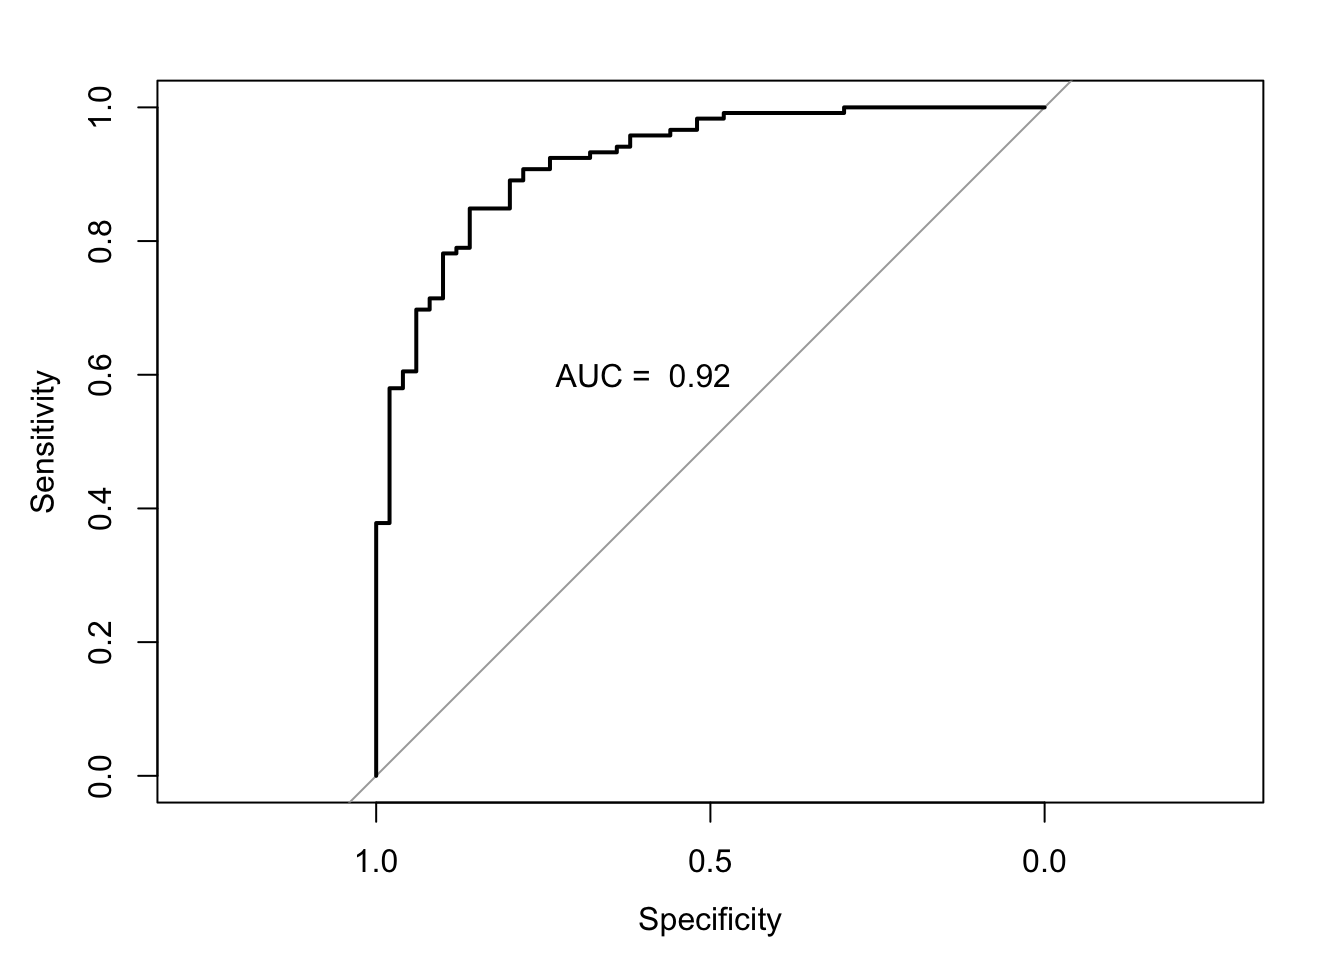
\includegraphics[keepaspectratio]{_main_files/figure-latex/unnamed-chunk-18-1.pdf}}

\section{Exercises}\label{lr.exerc}

\begin{enumerate}
\def\labelenumi{\arabic{enumi})}
\item
  The dataset \href{https://www.dropbox.com/s/vp44yozebx5xgok/bdiag.csv?dl=1}{bdiag.csv},
  included several imaging details from patients that had a biopsy to test for
  breast cancer.\\
  The variable \textbf{Diagnosis} classifies the biopsied tissue as M = malignant or
  B = benign.

  \begin{enumerate}
  \def\labelenumii{\alph{enumii})}
  \item
    Fit a logistic regression to predict \textbf{Diagnosis} using \textbf{texture\_mean}
    and \textbf{radius\_mean}.
  \item
    Build the confusion matrix for the model above
  \item
    Calculate the area and the ROC curve for the model in a).
  \item
    Plot the scatter plot for \textbf{texture\_mean}
    and \textbf{radius\_mean} and draw the border line for the prediction of
    \textbf{Diagnosis} based on the model in a)
  \item
    If you wanted to use the model above to predict the result of the biopsy,
    but wanted to decrease the chances of a false negative test, what strategy
    could you use?
  \end{enumerate}
\item
  The \href{https://www.dropbox.com/s/da3by5vuzkv77xi/SBI.csv?dl=1}{SBI.csv} dataset
  contains the information of more than 2300 children that attended the
  emergency services with fever and were tested for serious bacterial infection.
  The outcome \textbf{sbi} has 4 categories: Not Applicable(no infection) / UTI / Pneum / Bact

  \begin{enumerate}
  \def\labelenumii{\alph{enumii})}
  \item
    Build a multinomial model using \textbf{wcc}, \textbf{age}, \textbf{prevAB}, \textbf{pct},
    and \textbf{crp} to predict \textbf{sbi}
  \item
    Compute the confusion matrix and compute the kappa statistics
  \item
    How does the model classify a child with 1 year of age, WCC=29,
    PCT=5, CRP=200 and no prevAB?
  \end{enumerate}
\end{enumerate}

\chapter{Linear Discriminant Analysis}\label{linear-discriminant-analysis}

\section{Introduction}\label{lda.intro}

Once again we focus on \(\Pr (Y=k | X = x)\) to classify an individual (or other
unit) in one of the categories of \(Y\). Using the Bayes theorem,

\(\Pr (Y=k | X = x) = \frac{f_k(x) \Pr (Y=k) }{f(x)}\),

where \(f_k(x)\) is the density for \(X\mid Y=k\).

Thus, finding the category \(k\) that has the highest probability
\(\Pr (Y=k | X = x)\) is the same as finding the category \(k\) with higher value
for \(\frac{f_k(x)\Pr(Y=k) }{f(x)}\).

Now, if we assume that the density of \(X\) (represented above in a slight abuse
of notation as Pr(X=x)) is \(N(\mu, \sigma^2)\), it is possible to show that
maximising the right side of the equation is equivalent to maximising

\(\underbrace{x \cdot \frac{\mu_k}{\sigma^2} - \frac{\mu_k^2}{2\sigma^2} + \log\big(\Pr(Y=k)\big)}_{\text{discriminant function}}\)

So, if we get estimates for the parameters in the discriminant function,
we can calculate the category \(k\) that has the highest discriminant value and
thus the highest \(\Pr (Y=k | X = x)\).

\section{Readings}\label{lda.read}

Read the following chapters of \emph{An introduction to statistical learning}:

\begin{itemize}
\tightlist
\item
  4.4 Linear Discriminant Analysis
\item
  4.5 A Comparison of Classification Methods
\end{itemize}

\section{Practical session}\label{lda.prac}

\subsection*{Task 1 - Classification with the linear discriminant function}\label{task-1---classification-with-the-linear-discriminant-function}
\addcontentsline{toc}{subsection}{Task 1 - Classification with the linear discriminant function}

With the \href{https://www.dropbox.com/s/7wjsfdaf0wt2kg2/bmd.csv?dl=1}{bmd.csv}
dataset, let's use the variable \textbf{bmd} to predict \textbf{fracture} using linear
discriminant analysis.

The discriminant function is given by

\(age \cdot \frac{\mu_k}{\sigma^2} - \frac{\mu_k^2}{2\sigma^2} + \log\big(\Pr(Y=k)\big)\),

where \(\mu_k\) is the mean \textbf{bmd} for the group \(k=\) ``fracture'' or \(k=\)
``no fracture'', \(\sigma\) is the standard deviation for \textbf{bmd}, and \(\Pr(Y=k)\) is
the (marginal) probability of each category of the outcome.

We can easily get estimates for these parameters.

\begin{Shaded}
\begin{Highlighting}[]
\CommentTok{\#libraries that we will need}
\FunctionTok{library}\NormalTok{(MASS) }\CommentTok{\#lda function}
\FunctionTok{set.seed}\NormalTok{(}\DecValTok{1974}\NormalTok{) }\CommentTok{\#fix the random generator seed }

\CommentTok{\#read the data}
\NormalTok{bmd.data     }\OtherTok{\textless{}{-}} 
  \FunctionTok{read.csv}\NormalTok{(}\StringTok{"https://www.dropbox.com/s/c6mhgatkotuze8o/bmd.csv?dl=1"}\NormalTok{, }
           \AttributeTok{stringsAsFactors =} \ConstantTok{TRUE}\NormalTok{)}
\end{Highlighting}
\end{Shaded}

\begin{Shaded}
\begin{Highlighting}[]
\CommentTok{\#mean bmd for fracture}
\NormalTok{mean.f   }\OtherTok{\textless{}{-}} \FunctionTok{with}\NormalTok{(bmd.data, }\FunctionTok{mean}\NormalTok{(bmd[fracture}\SpecialCharTok{==}\StringTok{"fracture"}\NormalTok{]))  }
\CommentTok{\#mean bmd for no fracture}
\NormalTok{mean.nf  }\OtherTok{\textless{}{-}} \FunctionTok{with}\NormalTok{(bmd.data, }\FunctionTok{mean}\NormalTok{(bmd[fracture}\SpecialCharTok{==}\StringTok{"no fracture"}\NormalTok{])) }
\CommentTok{\#estimate of sigma (see page 141)}
\NormalTok{sigma.bmd }\OtherTok{\textless{}{-}} \FunctionTok{sqrt}\NormalTok{(}\FunctionTok{with}\NormalTok{(bmd.data,}
\NormalTok{                       (}\FunctionTok{sum}\NormalTok{((bmd[fracture}\SpecialCharTok{==}\StringTok{"fracture"}\NormalTok{] }\SpecialCharTok{{-}}\NormalTok{ mean.f)}\SpecialCharTok{\^{}}\DecValTok{2}\NormalTok{) }\SpecialCharTok{+}
                       \FunctionTok{sum}\NormalTok{((bmd[fracture}\SpecialCharTok{==}\StringTok{"no fracture"}\NormalTok{]}\SpecialCharTok{{-}}\NormalTok{ mean.nf)}\SpecialCharTok{\^{}}\DecValTok{2}\NormalTok{))}\SpecialCharTok{/}
\NormalTok{                    (}\FunctionTok{length}\NormalTok{(bmd)}\SpecialCharTok{{-}}\DecValTok{2}\NormalTok{)}
\NormalTok{                    )}
\NormalTok{                  )}
\CommentTok{\#probability of fracture/no fracture}
\NormalTok{pr.fracture }\OtherTok{\textless{}{-}} \FunctionTok{prop.table}\NormalTok{(}\FunctionTok{table}\NormalTok{(bmd.data}\SpecialCharTok{$}\NormalTok{fracture))}
    
\FunctionTok{print}\NormalTok{(}\FunctionTok{c}\NormalTok{(mean.f, mean.nf, sigma.bmd))}
\end{Highlighting}
\end{Shaded}

\begin{verbatim}
## [1] 0.6233080 0.8502454 0.1305394
\end{verbatim}

\begin{Shaded}
\begin{Highlighting}[]
\FunctionTok{print}\NormalTok{(pr.fracture)}
\end{Highlighting}
\end{Shaded}

\begin{verbatim}
## 
##    fracture no fracture 
##    0.295858    0.704142
\end{verbatim}

So, now we can compute the value of the discriminant function for a particular
\textbf{bmd}. For example, for \textbf{bmd}=0.54

\begin{Shaded}
\begin{Highlighting}[]
\CommentTok{\#for fracture}
\FloatTok{0.54}\SpecialCharTok{*}\NormalTok{mean.f}\SpecialCharTok{/}\NormalTok{sigma.bmd}\SpecialCharTok{\^{}}\DecValTok{2} \SpecialCharTok{{-}}\NormalTok{ mean.f}\SpecialCharTok{\^{}}\DecValTok{2}\SpecialCharTok{/}\NormalTok{(}\DecValTok{2}\SpecialCharTok{*}\NormalTok{sigma.bmd}\SpecialCharTok{\^{}}\DecValTok{2}\NormalTok{) }\SpecialCharTok{+} \FunctionTok{log}\NormalTok{(pr.fracture[}\DecValTok{1}\NormalTok{])      }
\end{Highlighting}
\end{Shaded}

\begin{verbatim}
## fracture 
## 7.134559
\end{verbatim}

\begin{Shaded}
\begin{Highlighting}[]
\CommentTok{\#for no fracture}
\FloatTok{0.54}\SpecialCharTok{*}\NormalTok{mean.nf}\SpecialCharTok{/}\NormalTok{sigma.bmd}\SpecialCharTok{\^{}}\DecValTok{2} \SpecialCharTok{{-}}\NormalTok{ mean.nf}\SpecialCharTok{\^{}}\DecValTok{2}\SpecialCharTok{/}\NormalTok{(}\DecValTok{2}\SpecialCharTok{*}\NormalTok{sigma.bmd}\SpecialCharTok{\^{}}\DecValTok{2}\NormalTok{) }\SpecialCharTok{+} \FunctionTok{log}\NormalTok{(pr.fracture[}\DecValTok{2}\NormalTok{])      }
\end{Highlighting}
\end{Shaded}

\begin{verbatim}
## no fracture 
##    5.381084
\end{verbatim}

Thus, for \textbf{bmd}=0.54, the classification would ``fracture'' given that this
category has the highest value for the discriminant function.

The linear discriminat analysis is implemented in the \texttt{lda()} function
from the \texttt{library(MASS)}

\begin{Shaded}
\begin{Highlighting}[]
\FunctionTok{library}\NormalTok{(MASS)}
\NormalTok{lda.model }\OtherTok{\textless{}{-}} \FunctionTok{lda}\NormalTok{(fracture}\SpecialCharTok{\textasciitilde{}}\NormalTok{bmd, }\AttributeTok{data=}\NormalTok{bmd.data)}

\CommentTok{\#to classify someone with bmd={-}.54 }
\CommentTok{\#}
\FunctionTok{predict}\NormalTok{(lda.model, }\AttributeTok{newdata=}\FunctionTok{data.frame}\NormalTok{(}\AttributeTok{bmd=}\FloatTok{0.54}\NormalTok{))}\SpecialCharTok{$}\NormalTok{class}
\end{Highlighting}
\end{Shaded}

\begin{verbatim}
## [1] fracture
## Levels: fracture no fracture
\end{verbatim}

\textbf{TRY IT YOURSELF:}

\begin{enumerate}
\def\labelenumi{\arabic{enumi})}
\tightlist
\item
  Compute the confusion matrix for LDA using \textbf{bmd} to
  predict \textbf{fracture}.
\end{enumerate}

\emph{See the solution code}

\begin{Shaded}
\begin{Highlighting}[]
 \CommentTok{\#predictions}
\NormalTok{pred.dataset }\OtherTok{\textless{}{-}} \FunctionTok{predict}\NormalTok{(lda.model)}\SpecialCharTok{$}\NormalTok{class}
\CommentTok{\#confusion matrix}
\FunctionTok{table}\NormalTok{(bmd.data}\SpecialCharTok{$}\NormalTok{fracture, pred.dataset)}
\end{Highlighting}
\end{Shaded}

\begin{enumerate}
\def\labelenumi{\arabic{enumi})}
\setcounter{enumi}{1}
\tightlist
\item
  Additionally to \textbf{bmd}, use \textbf{age}, \textbf{weight\_kg} and \textbf{height\_cm}, to
  predict \textbf{fracture} using LDA, and compute the confusion matrix. Compare the
  kappa statistic for this result with the one obtained in 1).
\end{enumerate}

\emph{See the solution code}

\begin{Shaded}
\begin{Highlighting}[]
\NormalTok{lda.model2 }\OtherTok{\textless{}{-}} \FunctionTok{lda}\NormalTok{(fracture}\SpecialCharTok{\textasciitilde{}}\NormalTok{bmd}\SpecialCharTok{+}\NormalTok{age}\SpecialCharTok{+}\NormalTok{weight\_kg}\SpecialCharTok{+}\NormalTok{height\_cm, }
                  \AttributeTok{data=}\NormalTok{bmd.data)}
\CommentTok{\#predictions}
\NormalTok{pred.dataset2 }\OtherTok{\textless{}{-}} \FunctionTok{predict}\NormalTok{(lda.model2)}\SpecialCharTok{$}\NormalTok{class}
\CommentTok{\#confusion matrix}
\FunctionTok{table}\NormalTok{(bmd.data}\SpecialCharTok{$}\NormalTok{fracture, pred.dataset2)}

\FunctionTok{library}\NormalTok{(irr) }\CommentTok{\#for the kappa statistics}
\end{Highlighting}
\end{Shaded}

\begin{verbatim}
## Loading required package: lpSolve
\end{verbatim}

\begin{Shaded}
\begin{Highlighting}[]
\FunctionTok{kappa2}\NormalTok{(}\FunctionTok{cbind}\NormalTok{(bmd.data}\SpecialCharTok{$}\NormalTok{fracture, pred.dataset))    }\CommentTok{\#model in 1)}
\FunctionTok{kappa2}\NormalTok{(}\FunctionTok{cbind}\NormalTok{(bmd.data}\SpecialCharTok{$}\NormalTok{fracture, pred.dataset2))   }\CommentTok{\#current model}
\end{Highlighting}
\end{Shaded}

\subsection*{Task 2 - Classification with the quadratic discriminant function}\label{task-2---classification-with-the-quadratic-discriminant-function}
\addcontentsline{toc}{subsection}{Task 2 - Classification with the quadratic discriminant function}

The linear discriminant function assumes that the variance is the
same for all the categories of the outcome. The quadratic discriminant
analysis (QDA) relaxes this assumption.

Let's repeat the classification of \textbf{fracture} with \textbf{bmd}, using a QDA

\begin{Shaded}
\begin{Highlighting}[]
\CommentTok{\#qda() is a function from the MASS}
\CommentTok{\#library that fits QDA}
\NormalTok{qda.model }\OtherTok{\textless{}{-}} \FunctionTok{qda}\NormalTok{(fracture }\SpecialCharTok{\textasciitilde{}}\NormalTok{ bmd, }
                  \AttributeTok{data=}\NormalTok{bmd.data)}
\end{Highlighting}
\end{Shaded}

We can now predict \textbf{fracture} for the individuals in the dataset and compare
it with the observed values (confusion matrix)

\begin{Shaded}
\begin{Highlighting}[]
\CommentTok{\#predictions}
\NormalTok{pred.qda }\OtherTok{\textless{}{-}} \FunctionTok{predict}\NormalTok{(qda.model)}\SpecialCharTok{$}\NormalTok{class}
\CommentTok{\#confusion matrix}
\FunctionTok{table}\NormalTok{(bmd.data}\SpecialCharTok{$}\NormalTok{fracture, pred.qda)}
\end{Highlighting}
\end{Shaded}

\begin{verbatim}
##              pred.qda
##               fracture no fracture
##   fracture          34          16
##   no fracture       10         109
\end{verbatim}

\textbf{TRY IT YOURSELF:}

\begin{enumerate}
\def\labelenumi{\arabic{enumi})}
\tightlist
\item
  Additionally to \textbf{bmd}, use \textbf{age}, \textbf{weight\_kg} and \textbf{height\_cm}, to
  predict \textbf{fracture} using QDA, and compute the confusion matrix.
\end{enumerate}

\emph{See the solution code}

\begin{Shaded}
\begin{Highlighting}[]
\NormalTok{qda.model2 }\OtherTok{\textless{}{-}} \FunctionTok{qda}\NormalTok{(fracture}\SpecialCharTok{\textasciitilde{}}\NormalTok{bmd}\SpecialCharTok{+}\NormalTok{age}\SpecialCharTok{+}\NormalTok{weight\_kg}\SpecialCharTok{+}\NormalTok{height\_cm, }
                  \AttributeTok{data=}\NormalTok{bmd.data)}
\CommentTok{\#predictions}
\NormalTok{pred.qda2 }\OtherTok{\textless{}{-}} \FunctionTok{predict}\NormalTok{(qda.model2)}\SpecialCharTok{$}\NormalTok{class}
\CommentTok{\#confusion matrix}
\FunctionTok{table}\NormalTok{(bmd.data}\SpecialCharTok{$}\NormalTok{fracture, pred.qda2)}
\end{Highlighting}
\end{Shaded}

\section{Exercises}\label{lda.exerc}

\begin{enumerate}
\def\labelenumi{\arabic{enumi})}
\item
  The dataset \href{https://www.dropbox.com/s/fvj7774lmyneab6/bdiag.csv?dl=1}{bdiag.csv},
  included several imaging details from patients that had a biopsy to test for
  breast cancer.\\
  The variable \textbf{Diagnosis} classifies the biopsied tissue as M = malignant or
  B = benign.

  \begin{enumerate}
  \def\labelenumii{\alph{enumii})}
  \item
    Use LDA to predict \textbf{Diagnosis} using \textbf{texture\_mean}
    and \textbf{radius\_mean}.
  \item
    Build the confusion matrix for the model above
  \item
    Compare the results with a logistic regession
  \item
    Plot the scatter plot for \textbf{texture\_mean}
    and \textbf{radius\_mean} and draw the border line for the prediction of
    \textbf{Diagnosis} based on the model in a)
  \item
    Use \textbf{radius\_mean, texture\_mean, perimeter\_mean, area\_mean,
    smoothness\_mean, compactness\_mean, symmetry\_mean,
    fractal\_dimension\_mean} to classify \textbf{diagnosis} with LDA and QDA.
    Check the distribution of the predictors.
  \end{enumerate}
\item
  Exercise 5 from the book (page 191)
\end{enumerate}

\chapter{K-nearest Neighbours Classification}\label{k-nearest-neighbours-classification}

\section{Introduction}\label{knnc.intro}

The K-nearest Neighbours (KNN) for classification, uses a similar idea to the
KNN regression. For KNN, a unit will be classified as the majority of its
neighbours.

\section{Readings}\label{knnc.read}

Read the following chapters of \emph{An introduction to statistical learning}:

\begin{itemize}
\tightlist
\item
  4.1 An Overview of Classification
\item
  2.2.3 The Classification Setting
\end{itemize}

\section{Practical session}\label{knnc.prac}

\subsection*{Task - KNN classification}\label{task---knn-classification}
\addcontentsline{toc}{subsection}{Task - KNN classification}

With the \href{https://www.dropbox.com/s/7wjsfdaf0wt2kg2/bmd.csv?dl=1}{bmd.csv}
dataset, we will use KNN (k=3) with the
variables AGE, SEX, BMI and BMD to
classify FRACTURE and compute the confusion matrix

First, let's import the dataset

\begin{Shaded}
\begin{Highlighting}[]
\CommentTok{\#libraries that we will need}
\FunctionTok{library}\NormalTok{(class)   }\CommentTok{\#knn }
\FunctionTok{set.seed}\NormalTok{(}\DecValTok{1974}\NormalTok{) }\CommentTok{\#fix the random generator seed }

\CommentTok{\#read the data}
\NormalTok{bmd.data     }\OtherTok{\textless{}{-}} 
  \FunctionTok{read.csv}\NormalTok{(}\StringTok{"https://www.dropbox.com/s/c6mhgatkotuze8o/bmd.csv?dl=1"}\NormalTok{, }
           \AttributeTok{stringsAsFactors =} \ConstantTok{TRUE}\NormalTok{)}
  
\NormalTok{bmd.data}\SpecialCharTok{$}\NormalTok{bmi }\OtherTok{\textless{}{-}}\NormalTok{ bmd.data}\SpecialCharTok{$}\NormalTok{weight\_kg }\SpecialCharTok{/}\NormalTok{ (bmd.data}\SpecialCharTok{$}\NormalTok{height\_cm}\SpecialCharTok{/}\DecValTok{100}\NormalTok{)}\SpecialCharTok{\^{}}\DecValTok{2}
\end{Highlighting}
\end{Shaded}

let's standardise all the variables so they have mean 0 and SD=1
so that the distances are in the same scale.

\begin{Shaded}
\begin{Highlighting}[]
\NormalTok{  bmd.data}\SpecialCharTok{$}\NormalTok{age.std     }\OtherTok{\textless{}{-}} \FunctionTok{scale}\NormalTok{(bmd.data}\SpecialCharTok{$}\NormalTok{age)}
\NormalTok{  bmd.data}\SpecialCharTok{$}\NormalTok{sex.num.std }\OtherTok{\textless{}{-}} \FunctionTok{scale}\NormalTok{(}\FunctionTok{as.numeric}\NormalTok{(bmd.data}\SpecialCharTok{$}\NormalTok{sex)) }\CommentTok{\#1{-}F, \#2{-}M}
\NormalTok{  bmd.data}\SpecialCharTok{$}\NormalTok{bmi.std     }\OtherTok{\textless{}{-}} \FunctionTok{scale}\NormalTok{(bmd.data}\SpecialCharTok{$}\NormalTok{bmi)  }
\NormalTok{  bmd.data}\SpecialCharTok{$}\NormalTok{bmd.std     }\OtherTok{\textless{}{-}} \FunctionTok{scale}\NormalTok{(bmd.data}\SpecialCharTok{$}\NormalTok{bmd) }
\end{Highlighting}
\end{Shaded}

Now we use knn=3

\begin{Shaded}
\begin{Highlighting}[]
\NormalTok{model.knn3 }\OtherTok{\textless{}{-}}  \FunctionTok{knn}\NormalTok{(}\AttributeTok{train =}\NormalTok{ bmd.data[}\FunctionTok{c}\NormalTok{(}\StringTok{"age.std"}\NormalTok{, }\StringTok{"sex.num.std"}\NormalTok{,}
                                      \StringTok{"bmi.std"}\NormalTok{,}\StringTok{"bmd.std"}\NormalTok{)],}
                   \AttributeTok{test  =}\NormalTok{ bmd.data[}\FunctionTok{c}\NormalTok{(}\StringTok{"age.std"}\NormalTok{, }\StringTok{"sex.num.std"}\NormalTok{,}
                                      \StringTok{"bmi.std"}\NormalTok{,}\StringTok{"bmd.std"}\NormalTok{)],}
                    \AttributeTok{cl    =}\NormalTok{ bmd.data}\SpecialCharTok{$}\NormalTok{fracture, }\AttributeTok{k=}\DecValTok{3}\NormalTok{)}
\FunctionTok{table}\NormalTok{(model.knn3, bmd.data}\SpecialCharTok{$}\NormalTok{fracture)}
\end{Highlighting}
\end{Shaded}

\begin{verbatim}
##              
## model.knn3    fracture no fracture
##   fracture          38           7
##   no fracture       12         112
\end{verbatim}

\textbf{TRY IT YOURSELF:}

\begin{enumerate}
\def\labelenumi{\arabic{enumi})}
\tightlist
\item
  Repeat the classification model from above but now with k=20 and
  compute the confusion matrix.
\end{enumerate}

\emph{See the solution code}

\begin{Shaded}
\begin{Highlighting}[]
\NormalTok{  model.knn20 }\OtherTok{\textless{}{-}}  \FunctionTok{knn}\NormalTok{(}\AttributeTok{train =}\NormalTok{ bmd.data[}\FunctionTok{c}\NormalTok{(}\StringTok{"age.std"}\NormalTok{, }\StringTok{"sex.num.std"}\NormalTok{,}
                                        \StringTok{"bmi.std"}\NormalTok{,}\StringTok{"bmd.std"}\NormalTok{)],}
                   \AttributeTok{test  =}\NormalTok{ bmd.data[}\FunctionTok{c}\NormalTok{(}\StringTok{"age.std"}\NormalTok{, }\StringTok{"sex.num.std"}\NormalTok{,}
                                         \StringTok{"bmi.std"}\NormalTok{,}\StringTok{"bmd.std"}\NormalTok{)],}
                    \AttributeTok{cl    =}\NormalTok{ bmd.data}\SpecialCharTok{$}\NormalTok{fracture, }\AttributeTok{k=}\DecValTok{20}\NormalTok{ )}
  \FunctionTok{table}\NormalTok{(model.knn20, bmd.data}\SpecialCharTok{$}\NormalTok{fracture)}
\end{Highlighting}
\end{Shaded}

\begin{enumerate}
\def\labelenumi{\arabic{enumi})}
\setcounter{enumi}{1}
\tightlist
\item
  (advanced) Plot the error rate for KNN with k=1 to 20 using the
  variables AGE, SEX, BMI and BMD to classify FRACTURE
\end{enumerate}

\emph{See the solution code}

\begin{Shaded}
\begin{Highlighting}[]
\NormalTok{knn.fit }\OtherTok{\textless{}{-}} \ControlFlowTok{function}\NormalTok{(k.par)\{}
\NormalTok{  knn.model }\OtherTok{\textless{}{-}} \FunctionTok{knn}\NormalTok{(}\AttributeTok{train =}\NormalTok{ bmd.data[}\FunctionTok{c}\NormalTok{(}\StringTok{"age.std"}\NormalTok{, }\StringTok{"sex.num.std"}\NormalTok{,}
                                      \StringTok{"bmi.std"}\NormalTok{,}\StringTok{"bmd.std"}\NormalTok{)],}
                   \AttributeTok{test  =}\NormalTok{ bmd.data[}\FunctionTok{c}\NormalTok{(}\StringTok{"age.std"}\NormalTok{, }\StringTok{"sex.num.std"}\NormalTok{,}
                                      \StringTok{"bmi.std"}\NormalTok{,}\StringTok{"bmd.std"}\NormalTok{)],}
                    \AttributeTok{cl    =}\NormalTok{ bmd.data}\SpecialCharTok{$}\NormalTok{fracture, }\AttributeTok{k=}\NormalTok{k.par )}
\NormalTok{  class.error}\OtherTok{\textless{}{-}} \DecValTok{1}\SpecialCharTok{{-}}\FunctionTok{sum}\NormalTok{(}\FunctionTok{diag}\NormalTok{(}\FunctionTok{table}\NormalTok{( knn.model, bmd.data}\SpecialCharTok{$}\NormalTok{fracture))}\SpecialCharTok{/}\DecValTok{169}\NormalTok{)}
  \FunctionTok{return}\NormalTok{(class.error)}
\NormalTok{\}}

\NormalTok{  class.error1to20 }\OtherTok{\textless{}{-}} \FunctionTok{sapply}\NormalTok{(}\FunctionTok{seq}\NormalTok{(}\DecValTok{1}\NormalTok{,}\DecValTok{20}\NormalTok{), knn.fit)}
  \FunctionTok{plot}\NormalTok{(}\FunctionTok{seq}\NormalTok{(}\DecValTok{1}\NormalTok{,}\DecValTok{20}\NormalTok{), class.error1to20, }\AttributeTok{type=}\StringTok{"l"}\NormalTok{)}
\end{Highlighting}
\end{Shaded}

\pandocbounded{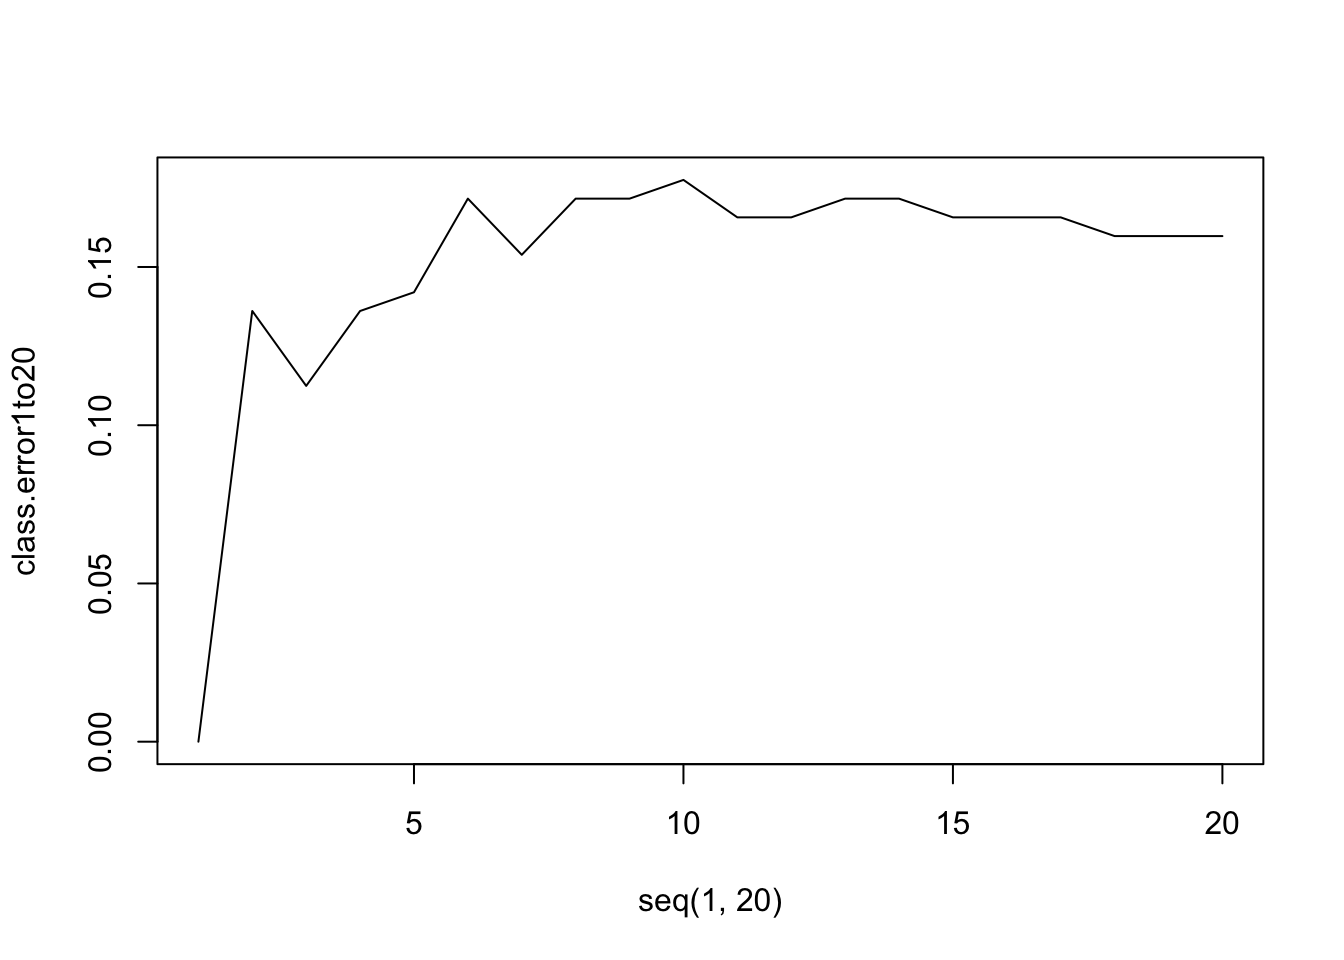
\includegraphics[keepaspectratio]{_main_files/figure-latex/unnamed-chunk-33-1.pdf}}

\section{Exercises}\label{knnc.exerc}

\begin{enumerate}
\def\labelenumi{\arabic{enumi})}
\item
  The dataset \href{https://www.dropbox.com/s/fvj7774lmyneab6/bdiag.csv?dl=1}{bdiag.csv},
  included several imaging details from patients that had a biopsy to test for
  breast cancer.\\
  The variable \textbf{diagnosis} classifies the biopsied tissue as M = malignant or
  B = benign.

  \begin{enumerate}
  \def\labelenumii{\alph{enumii})}
  \item
    Use a KNN with k=5 to predict \textbf{Diagnosis} using \textbf{texture\_mean}
    and \textbf{radius\_mean}.
  \item
    Build the confusion matrix for the classification above
  \item
    Plot the scatter plot for \textbf{texture\_mean}
    and \textbf{radius\_mean} and draw the border line for the prediction of
    \textbf{Diagnosis} based on the model in a)
  \item
    Plot the scatter plot for \textbf{texture\_mean}
    and \textbf{radius\_mean} and draw the border line for the prediction of
    \textbf{Diagnosis} based knn, k=15
  \end{enumerate}
\end{enumerate}

\end{document}
